\documentclass[12pt, a4paper]{book}
\begin{document}

\chapter{Kinematical variables distribution in control region}\label{apendix:Kin_var_in_CR}
\graphicspath{{../../Plots/Data_Analysis/SRs/Control_region/}} 
\begin{figure}[!ht]
    \centering
    \begin{subfigure}[b]{0.49\textwidth}
        \centering
        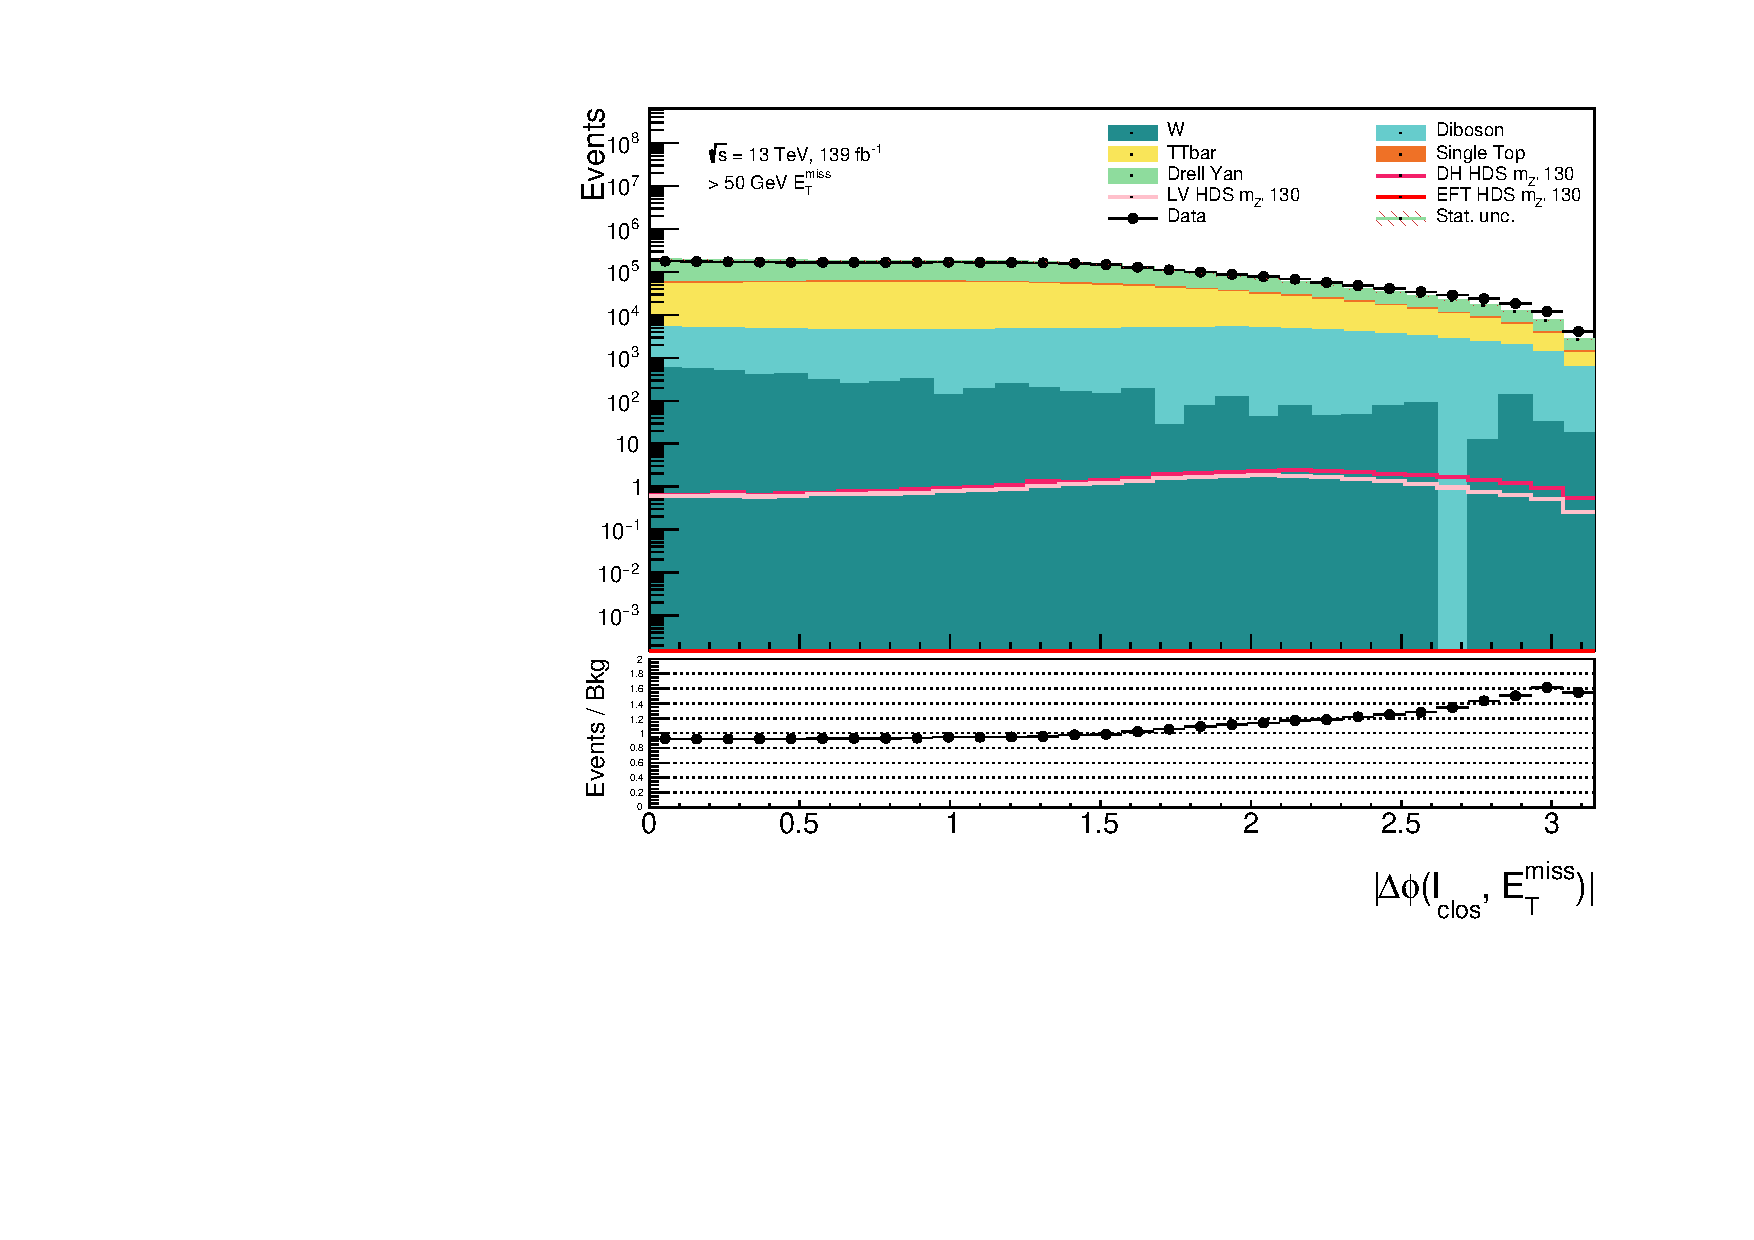
\includegraphics[width=\textwidth]{dPhiCloseMet.pdf}
    \end{subfigure}
    \hfill
    \begin{subfigure}[b]{0.49\textwidth}
        \centering
        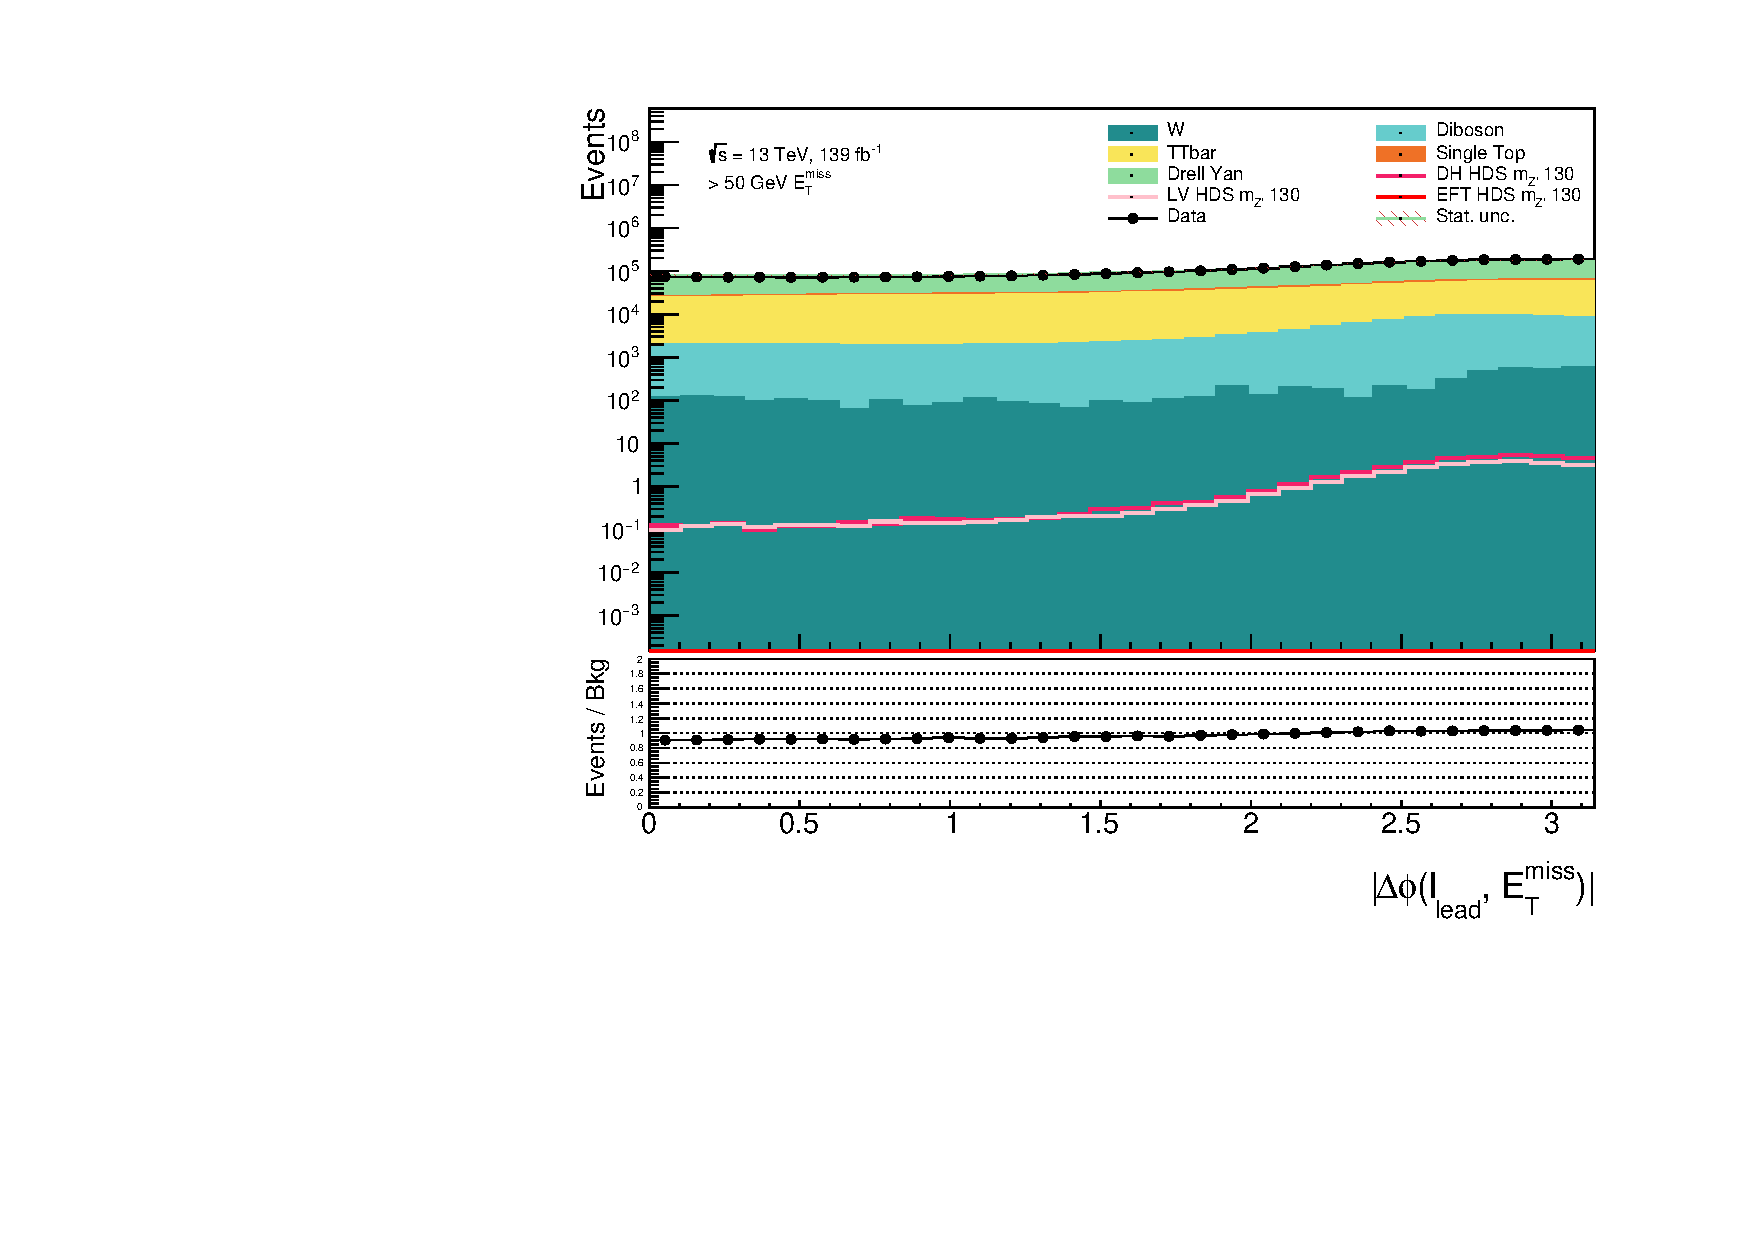
\includegraphics[width=\textwidth]{dPhiLeadMet.pdf}
    \end{subfigure}
    \begin{subfigure}[b]{0.49\textwidth}
        \centering
        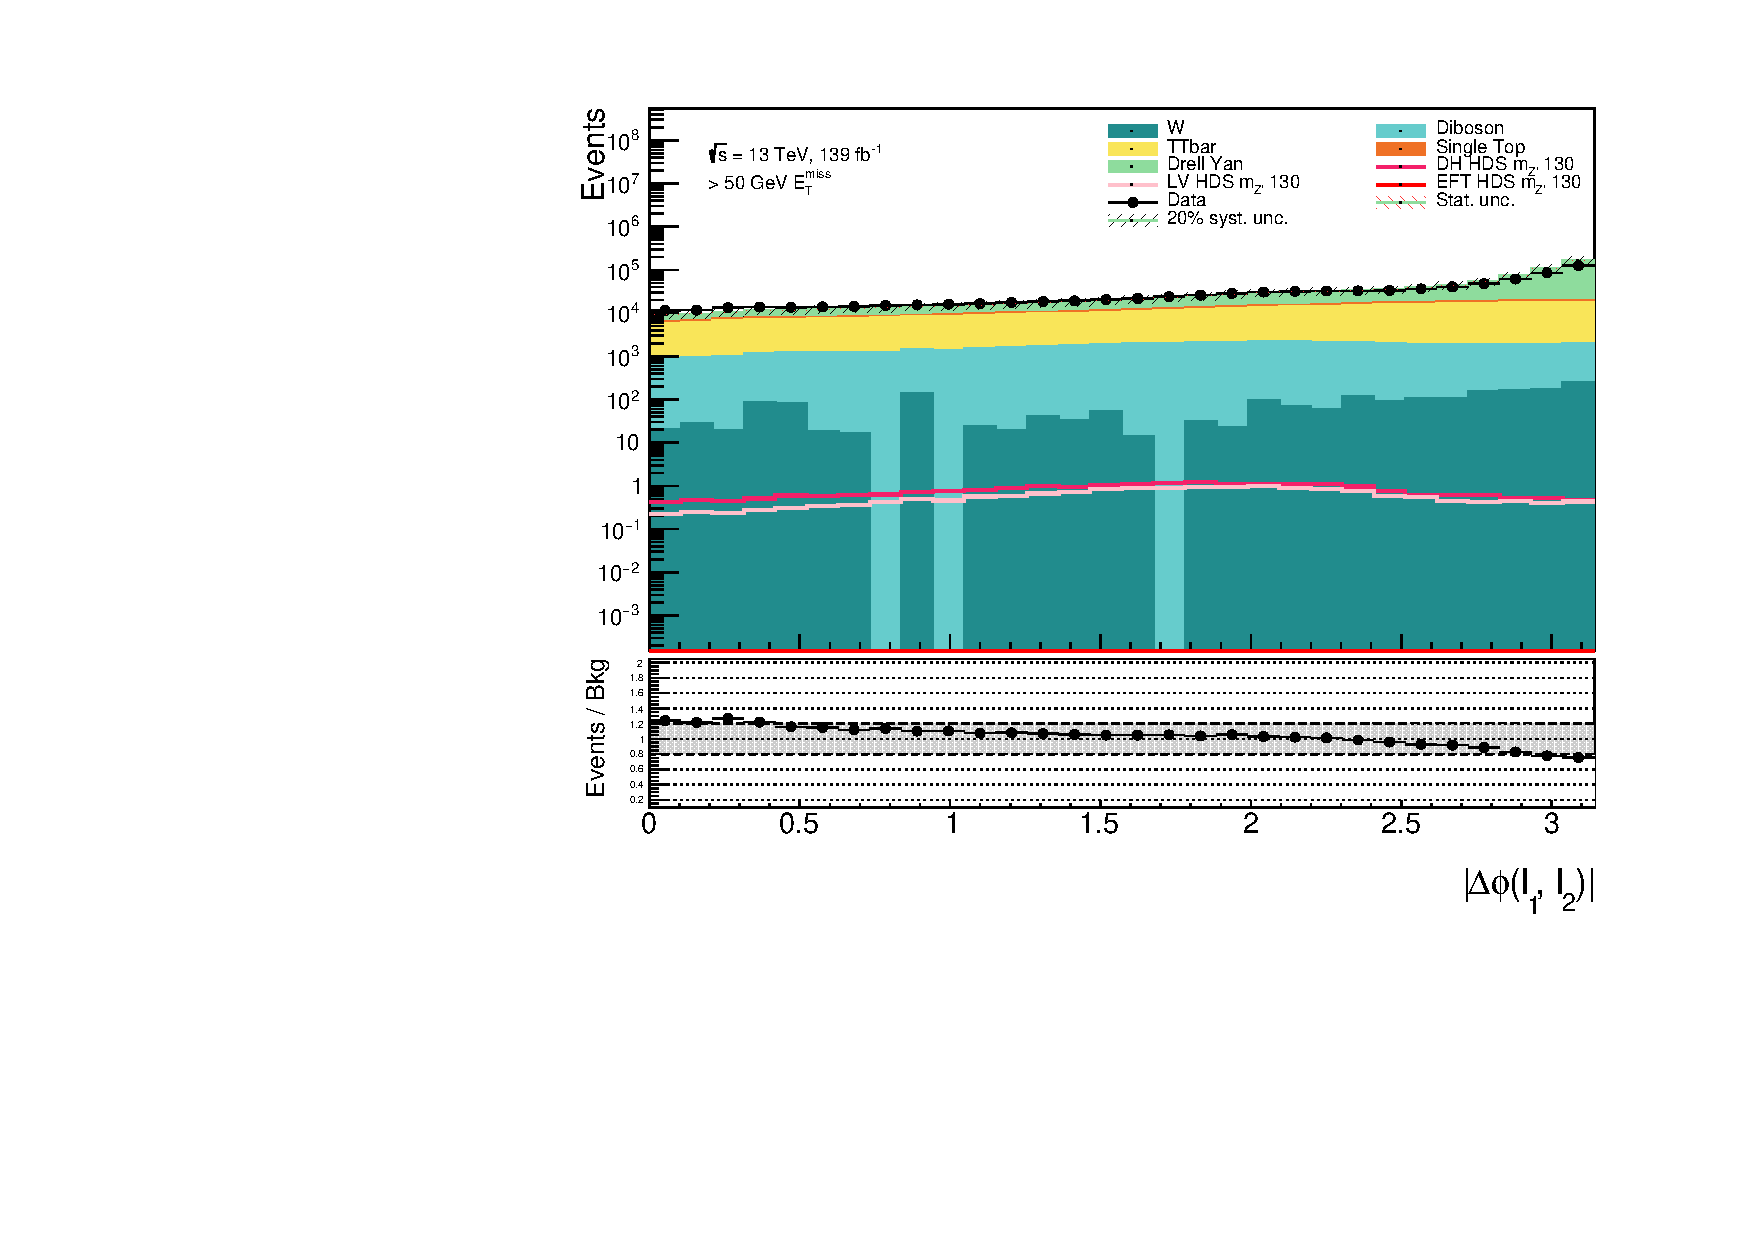
\includegraphics[width=\textwidth]{dPhiLeps.pdf}
    \end{subfigure}
    \begin{subfigure}[b]{0.49\textwidth}
        \centering
        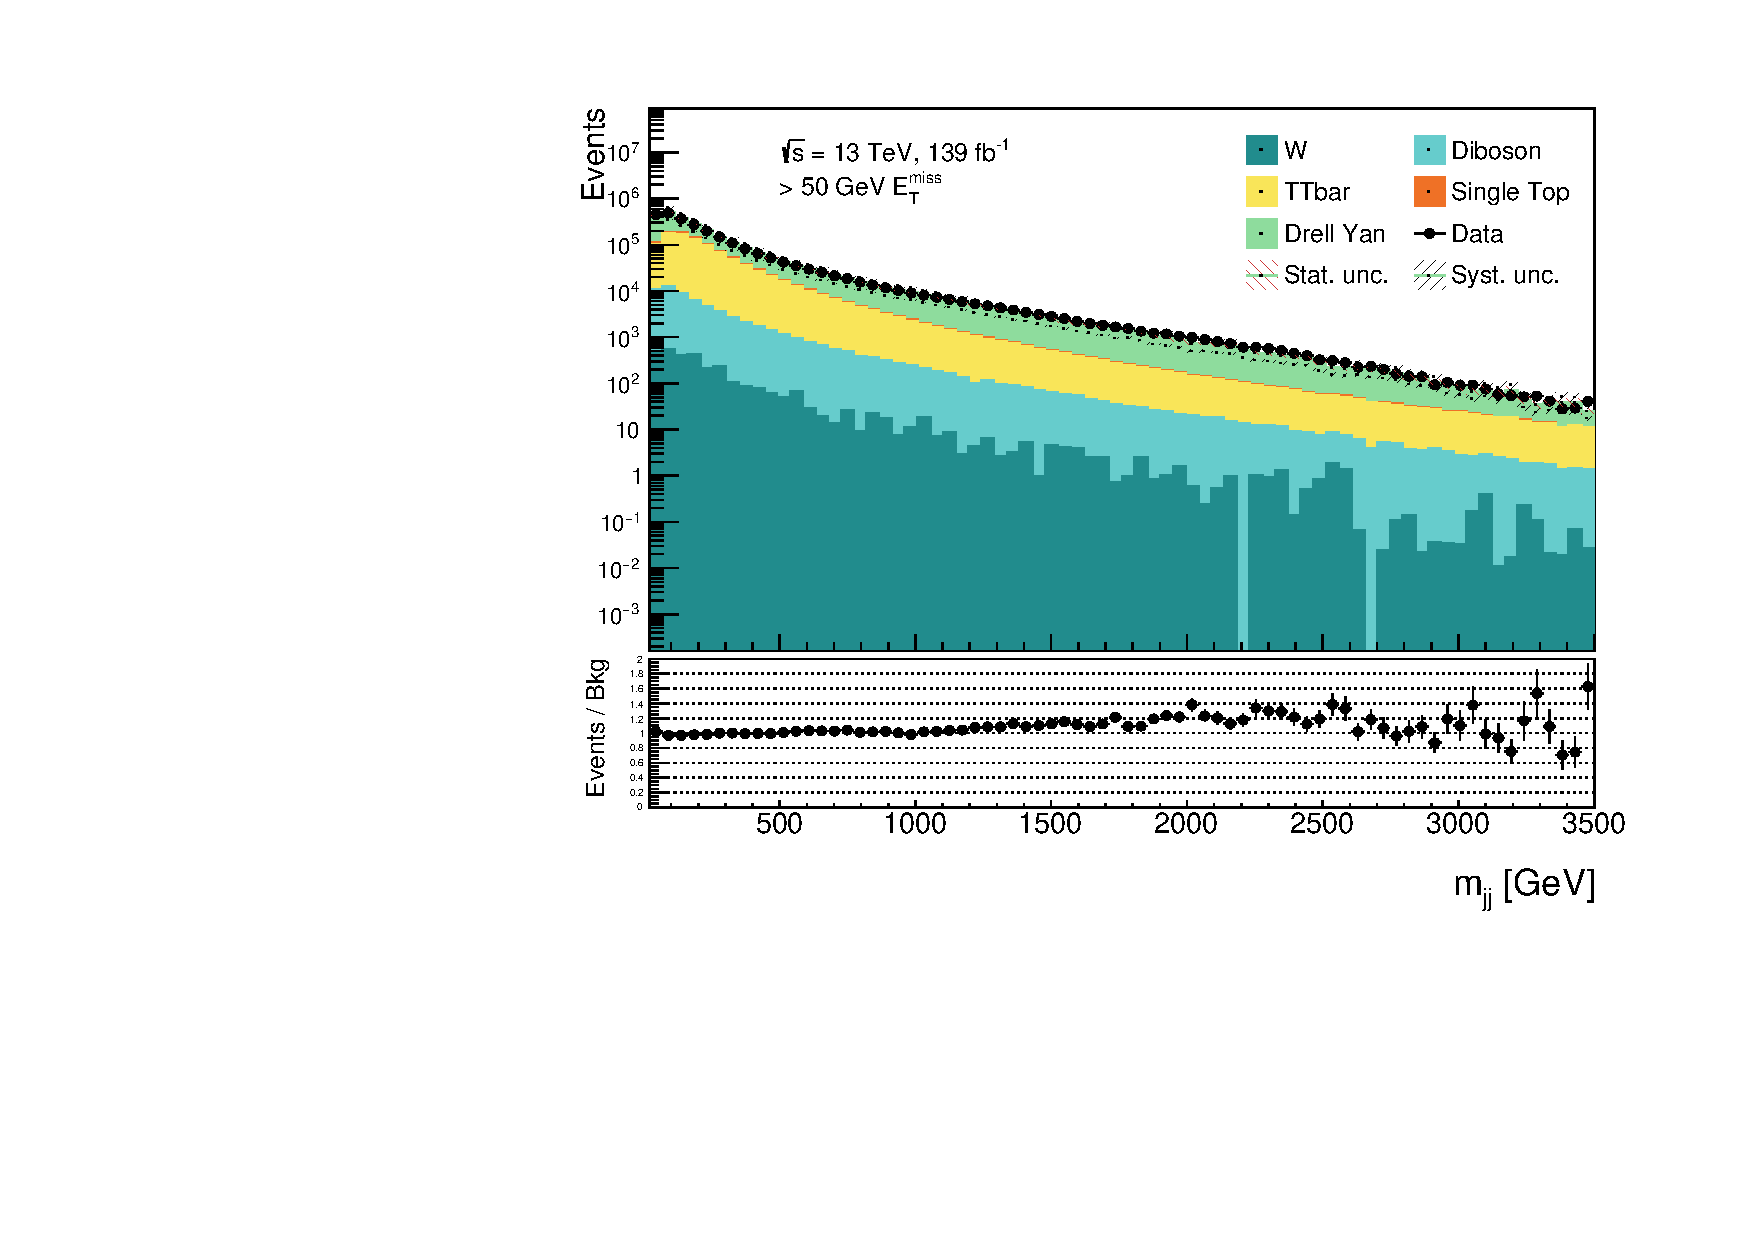
\includegraphics[width=\textwidth]{mjj.pdf}
    \end{subfigure}
    \caption{$\Delta\phi(l_c,E_T^{miss})$, $\Delta\phi(l_l,E_T^{miss})$, $\Delta\phi(l_1,l_2)$ and $m_{jj}$ distribution in the control region.}
\end{figure}
\begin{figure}[!ht]
    \centering
    \begin{subfigure}[b]{0.49\textwidth}
        \centering
        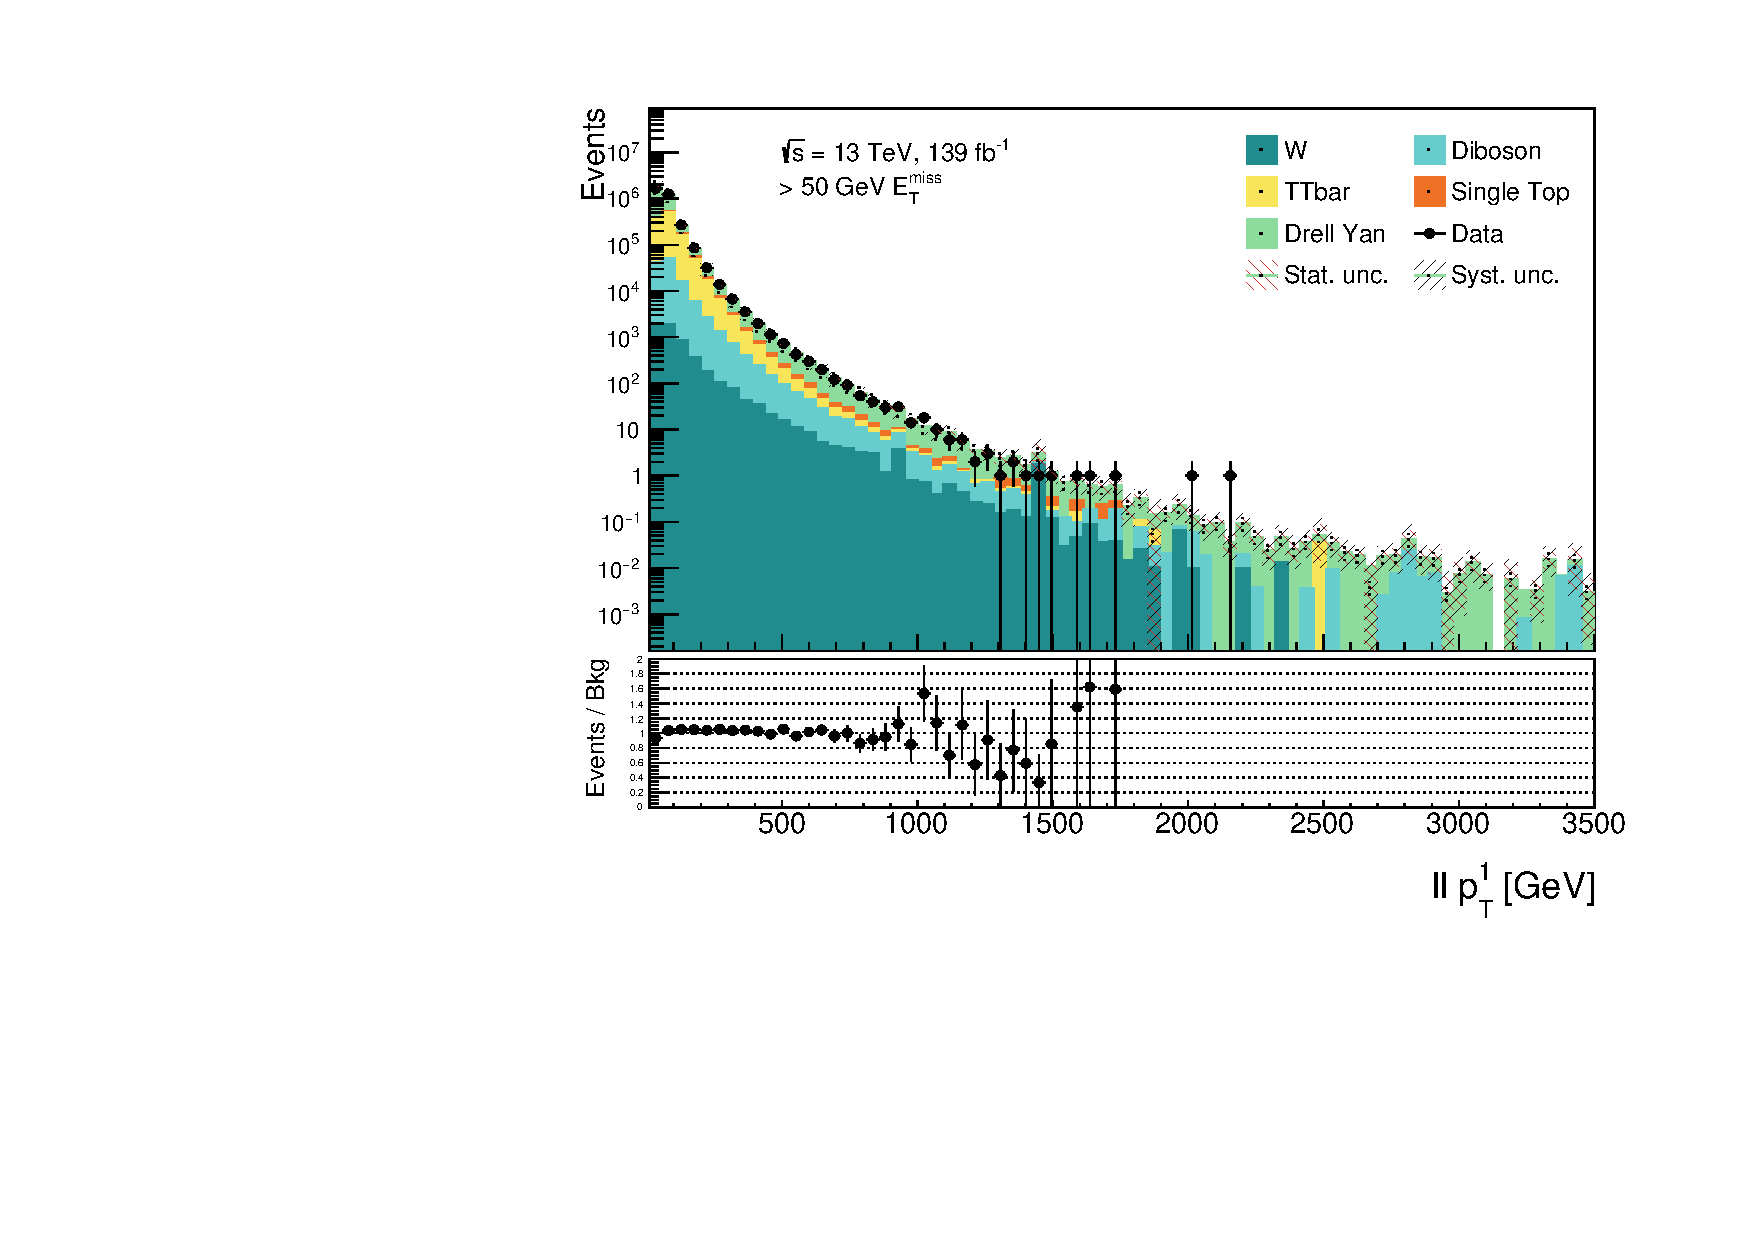
\includegraphics[width=\textwidth]{pt1_ll.pdf}
    \end{subfigure}
    \hfill
    \begin{subfigure}[b]{0.49\textwidth}
        \centering
        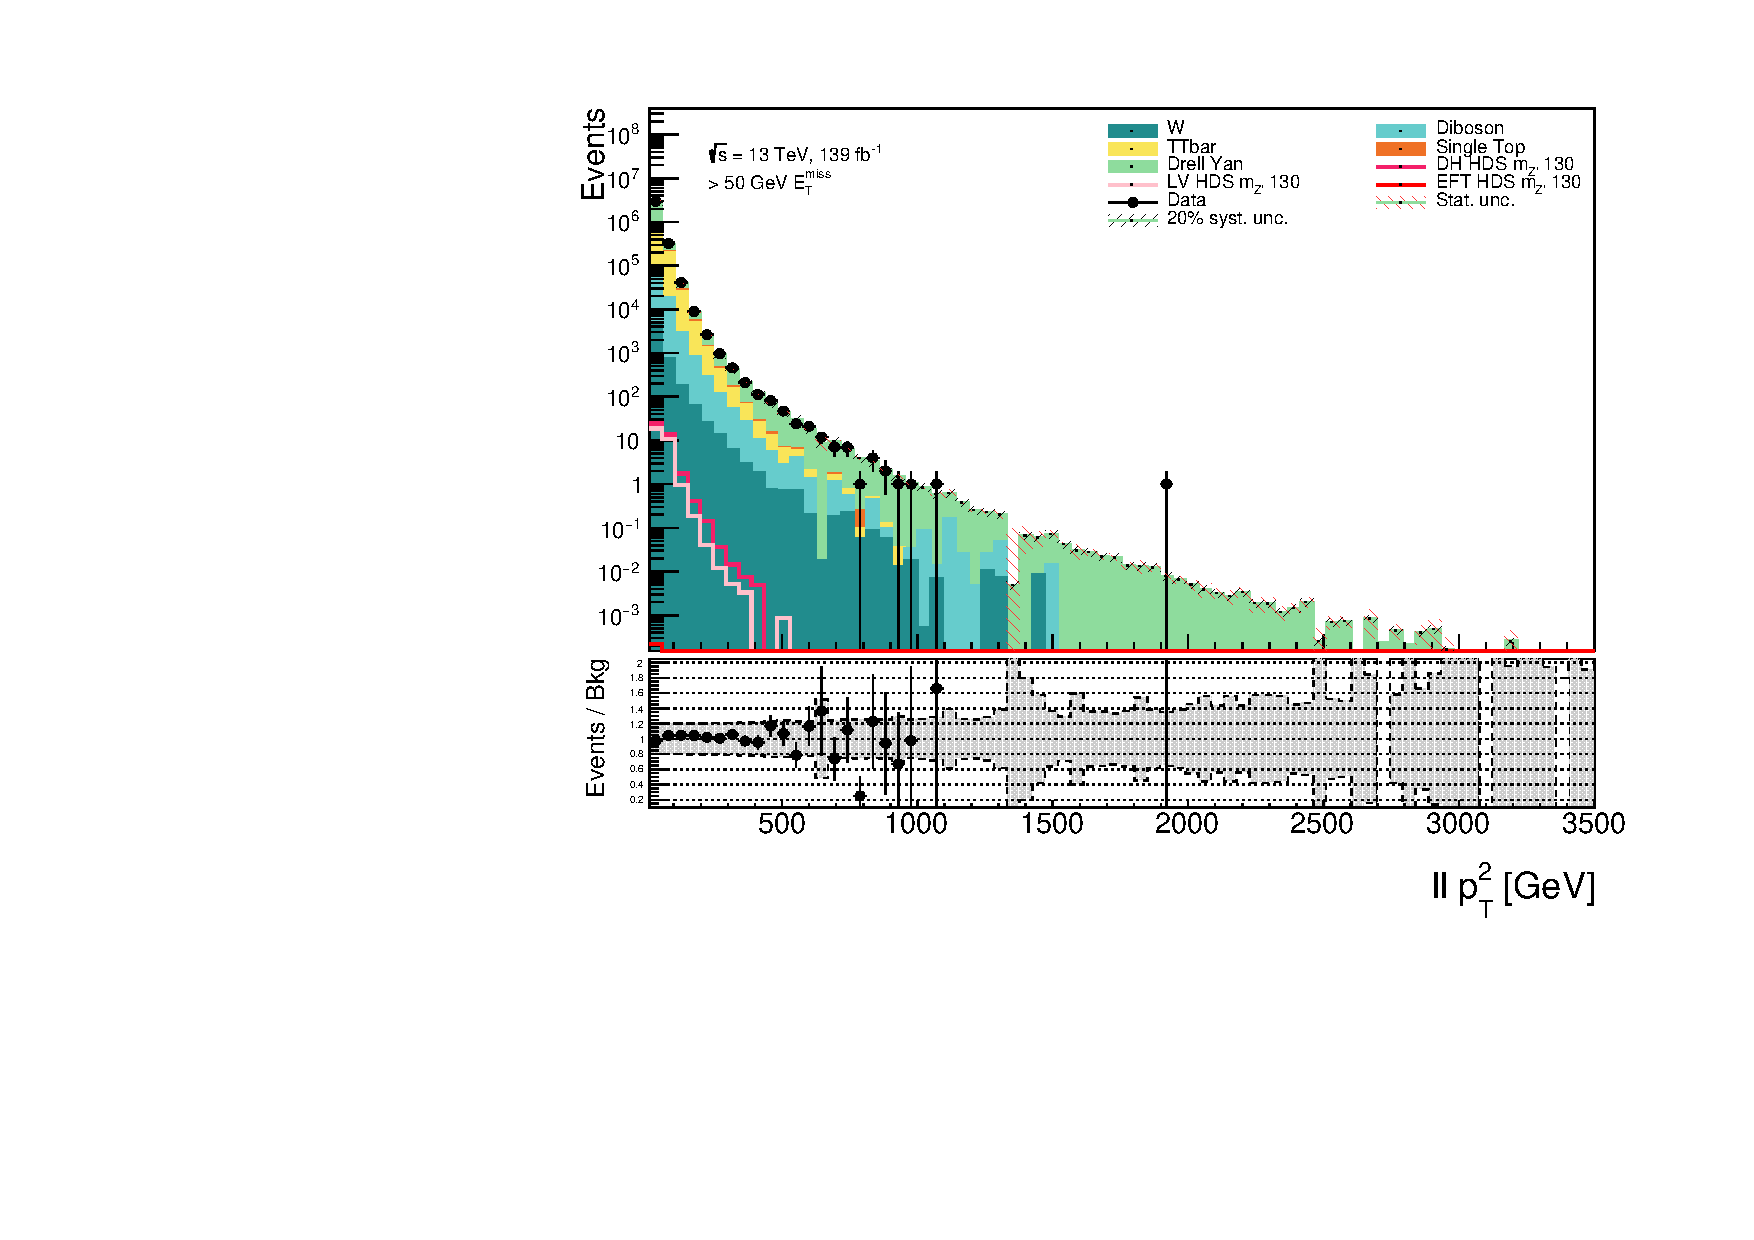
\includegraphics[width=\textwidth]{pt2_ll.pdf}
    \end{subfigure}
    \begin{subfigure}[b]{0.49\textwidth}
        \centering
        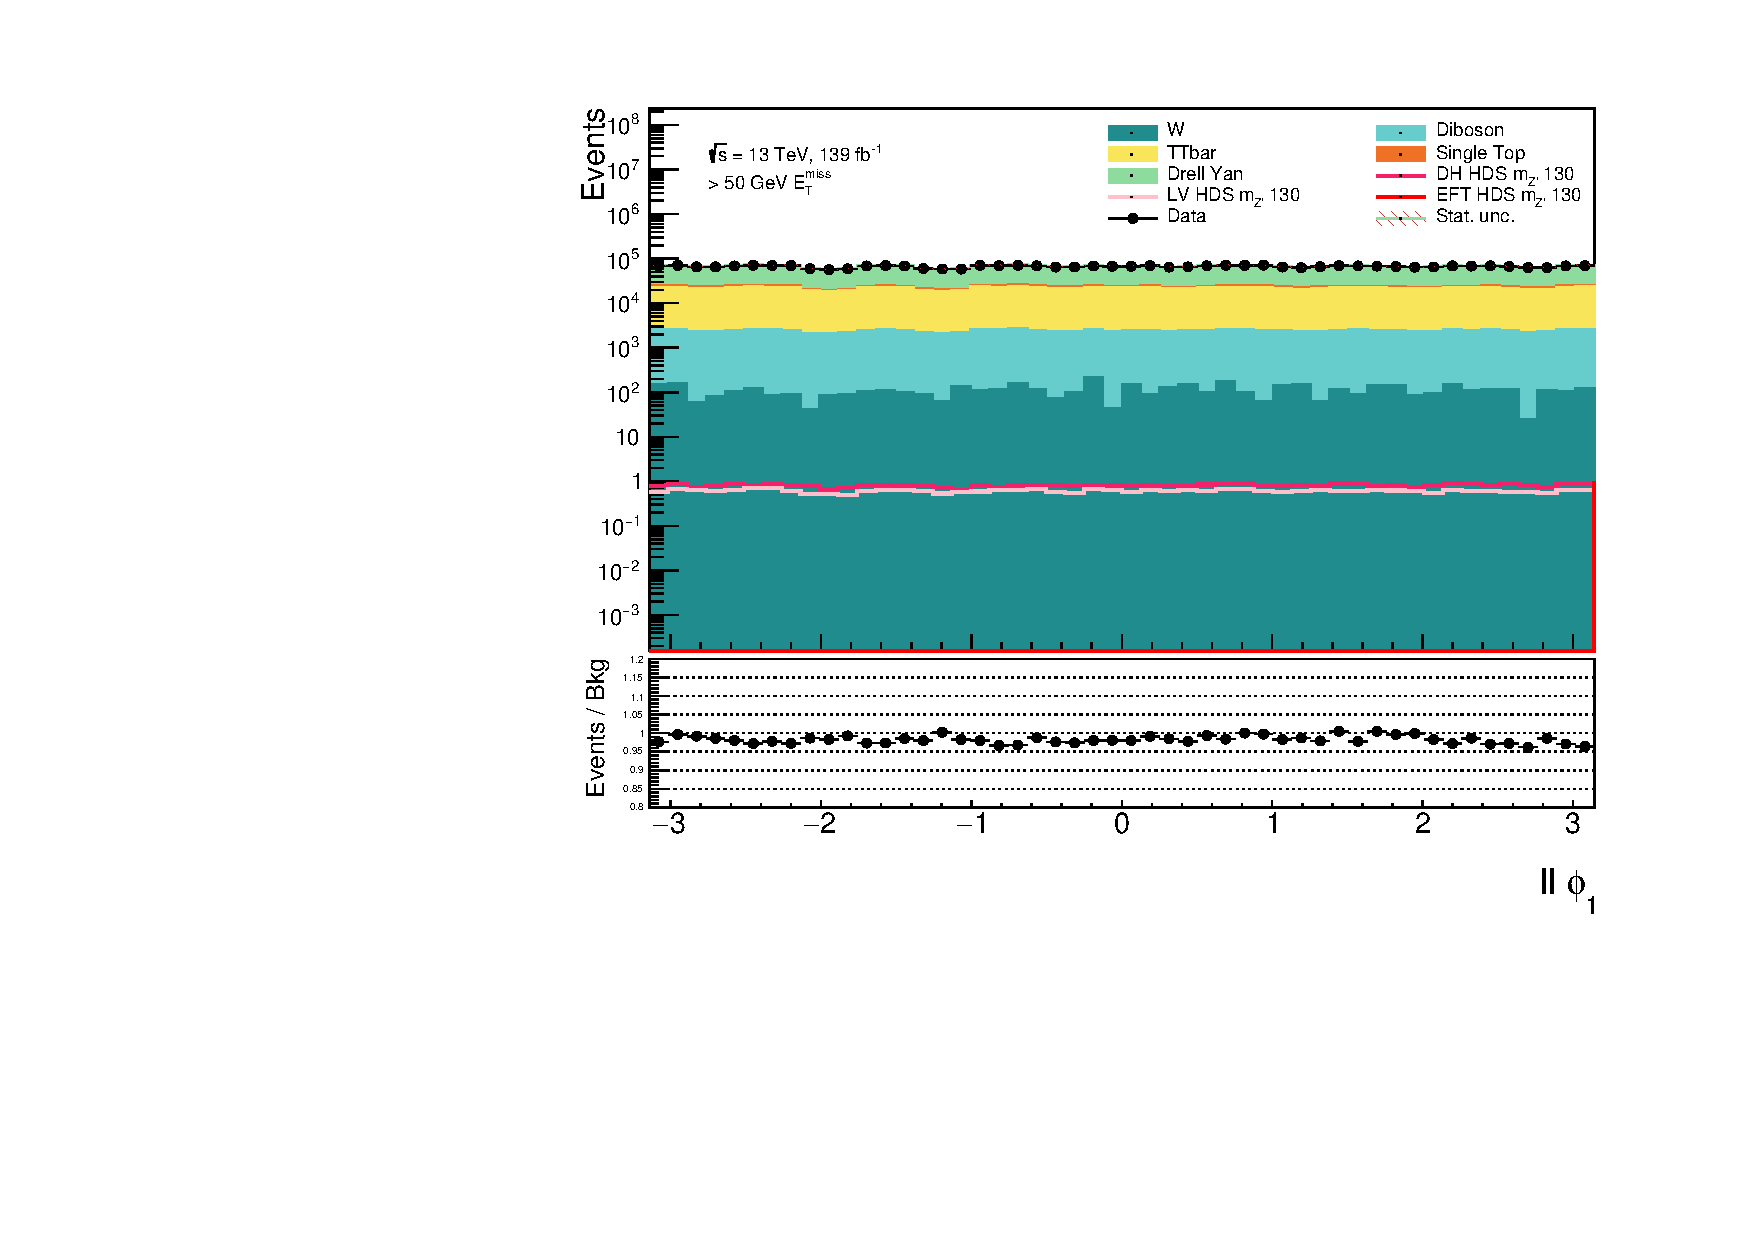
\includegraphics[width=\textwidth]{phi1_ll.pdf}
    \end{subfigure}
    \hfill
    \begin{subfigure}[b]{0.49\textwidth}
        \centering
        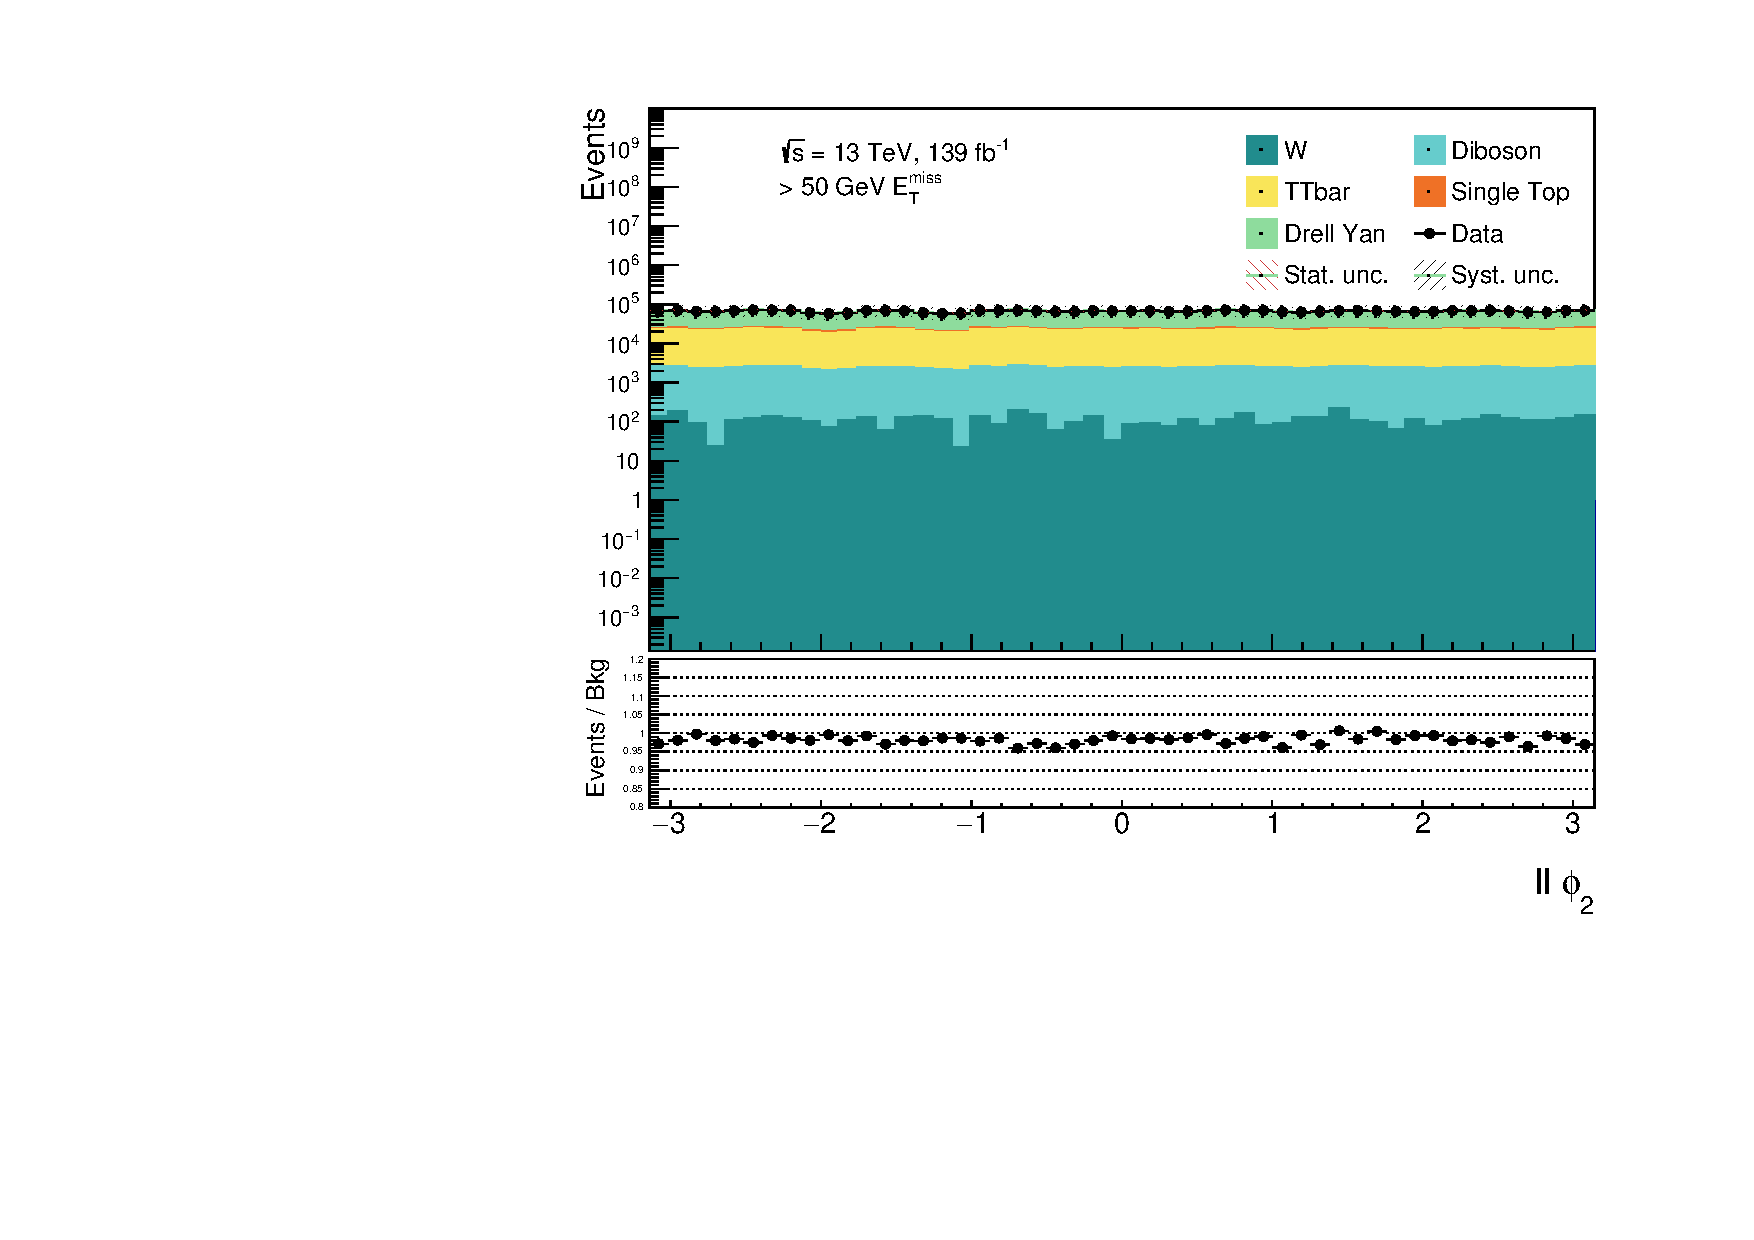
\includegraphics[width=\textwidth]{phi2_ll.pdf}
    \end{subfigure}
    \begin{subfigure}[b]{0.49\textwidth}
        \centering
        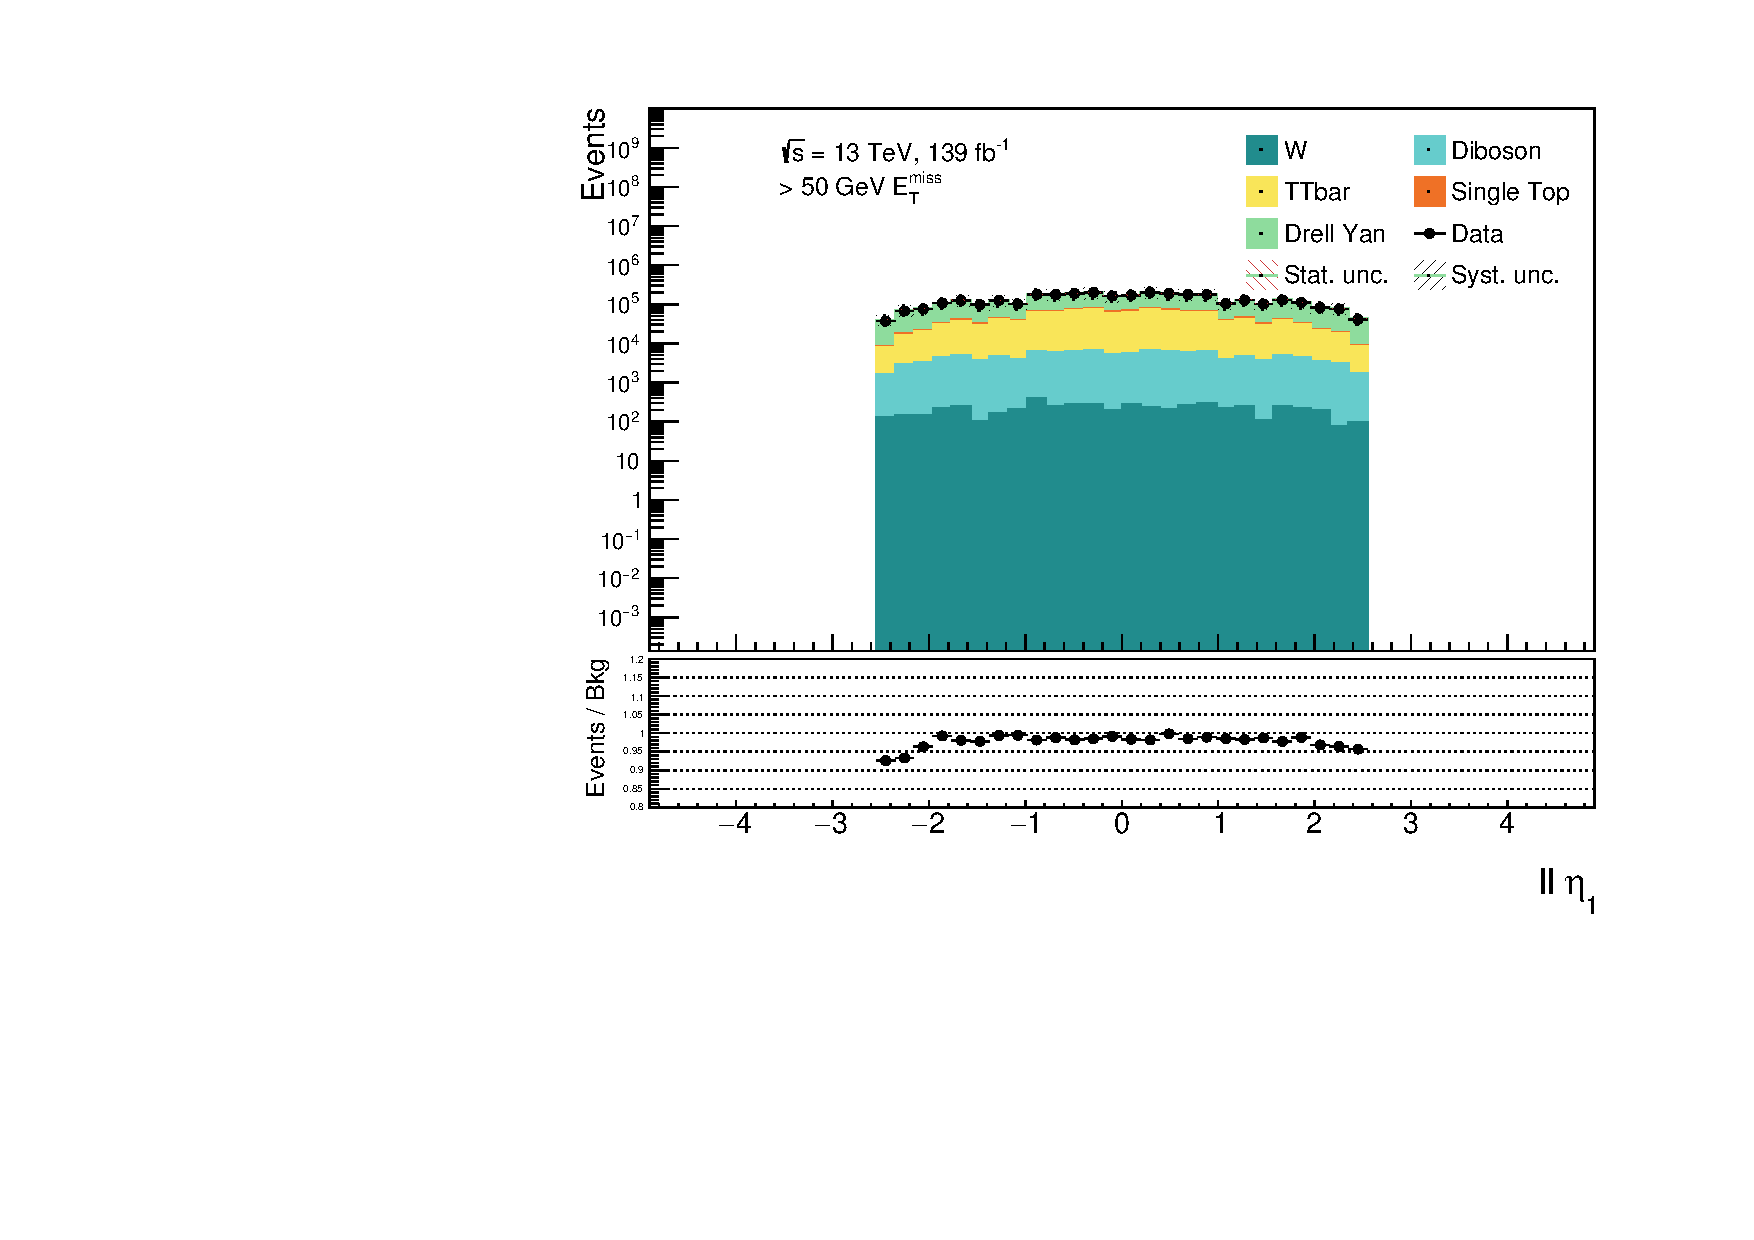
\includegraphics[width=\textwidth]{eta1_ll.pdf}
    \end{subfigure}
    \hfill
    \begin{subfigure}[b]{0.49\textwidth}
        \centering
        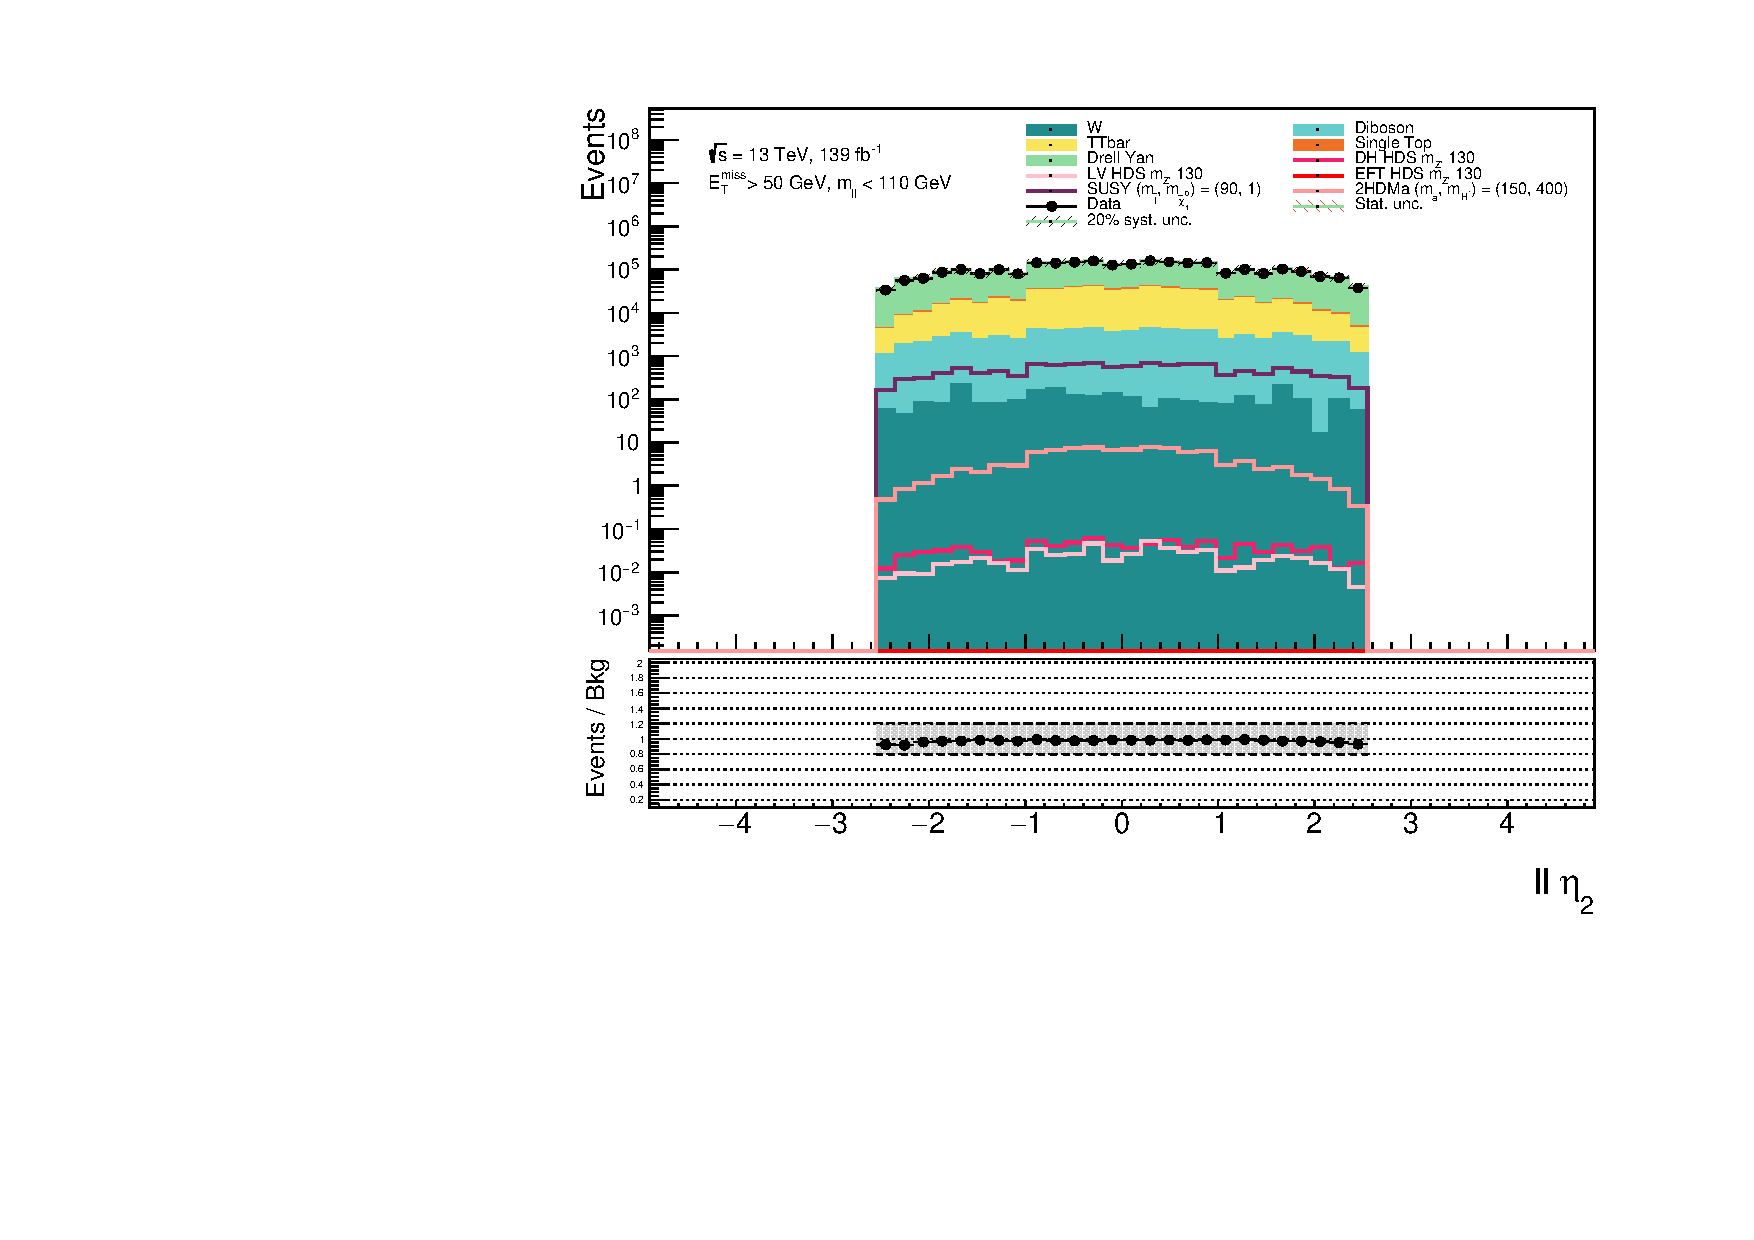
\includegraphics[width=\textwidth]{eta2_ll.pdf}
    \end{subfigure}
    \caption{Leptons $p_T, \phi$ and $\eta$ distribution in the control region.}
\end{figure}
\begin{figure}[!ht]
    \centering
    \begin{subfigure}[b]{0.49\textwidth}
        \centering
        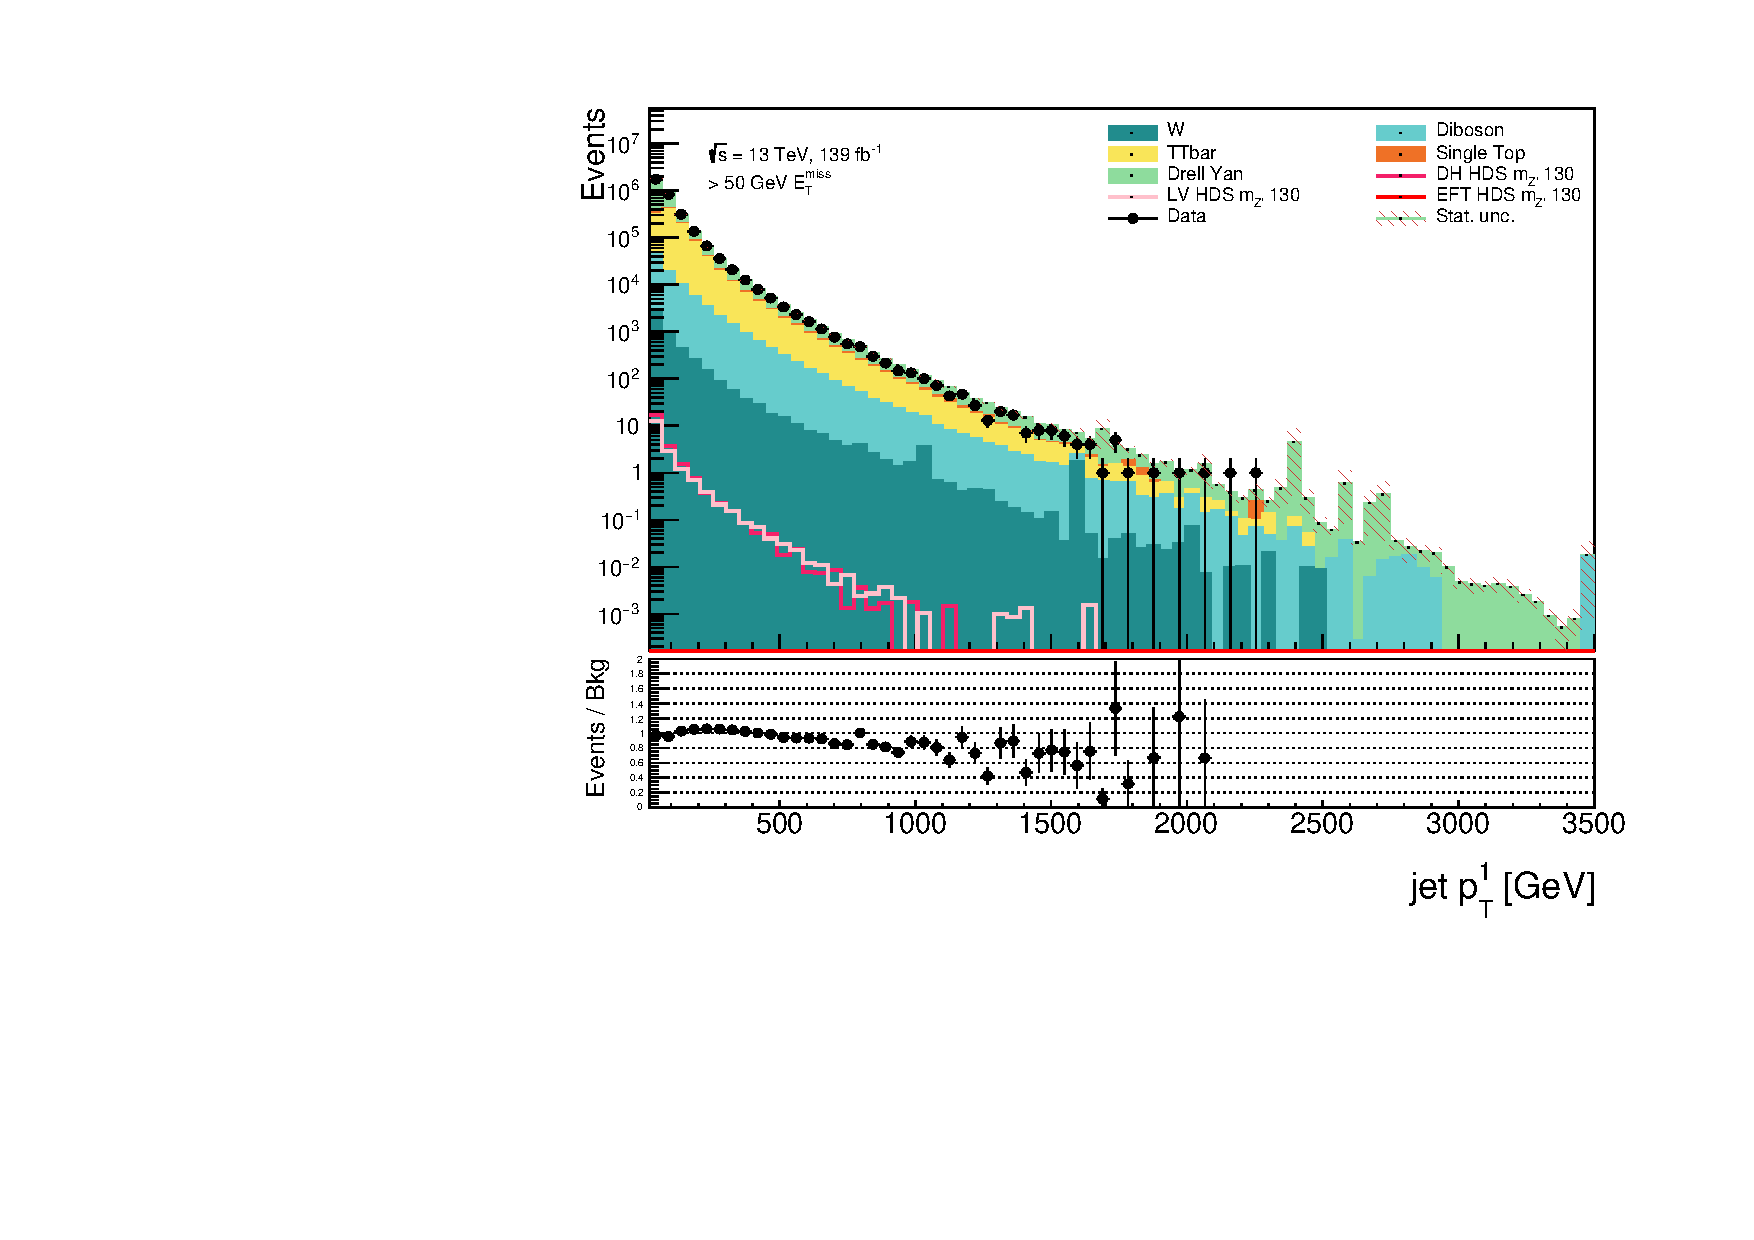
\includegraphics[width=\textwidth]{pt1_jet.pdf}
    \end{subfigure}
    \hfill
    \begin{subfigure}[b]{0.49\textwidth}
        \centering
        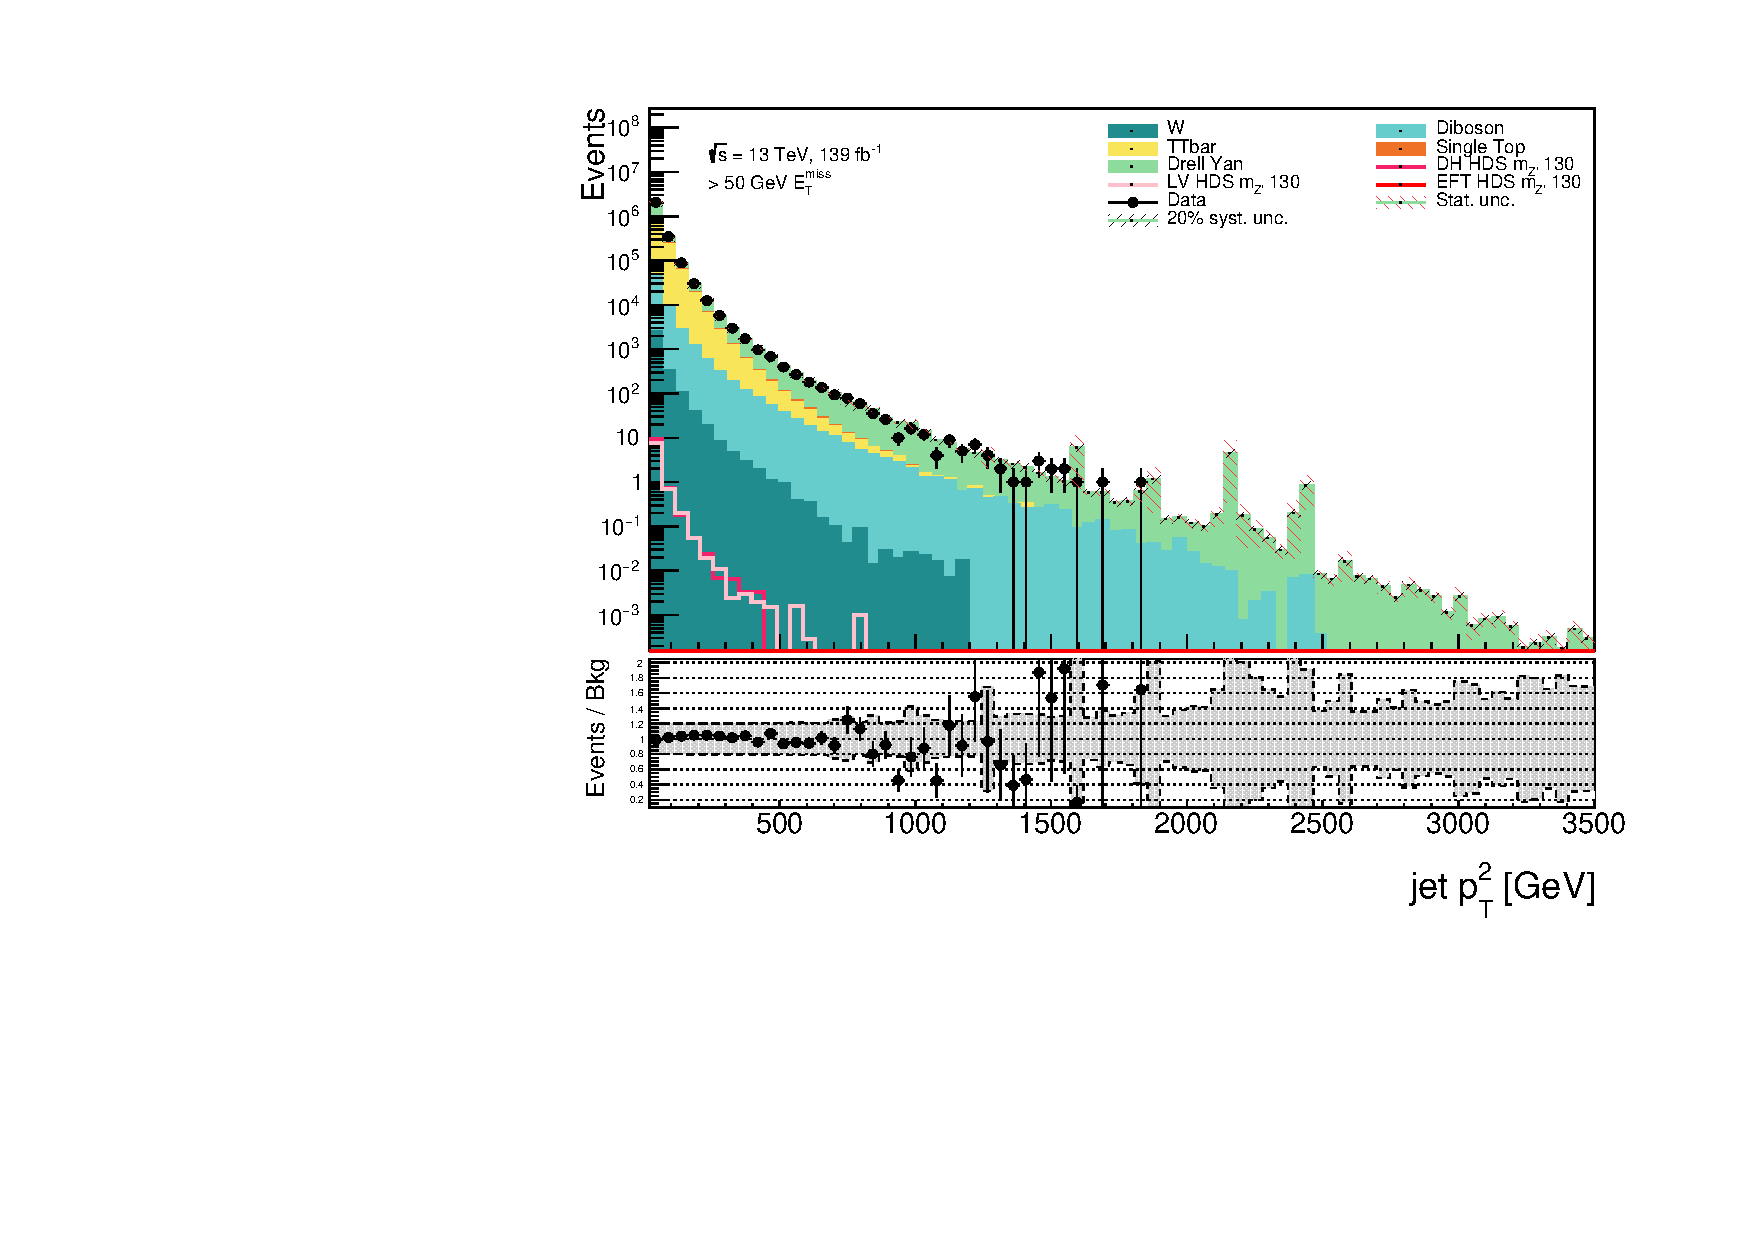
\includegraphics[width=\textwidth]{pt2_jet.pdf}
    \end{subfigure}
    \begin{subfigure}[b]{0.49\textwidth}
        \centering
        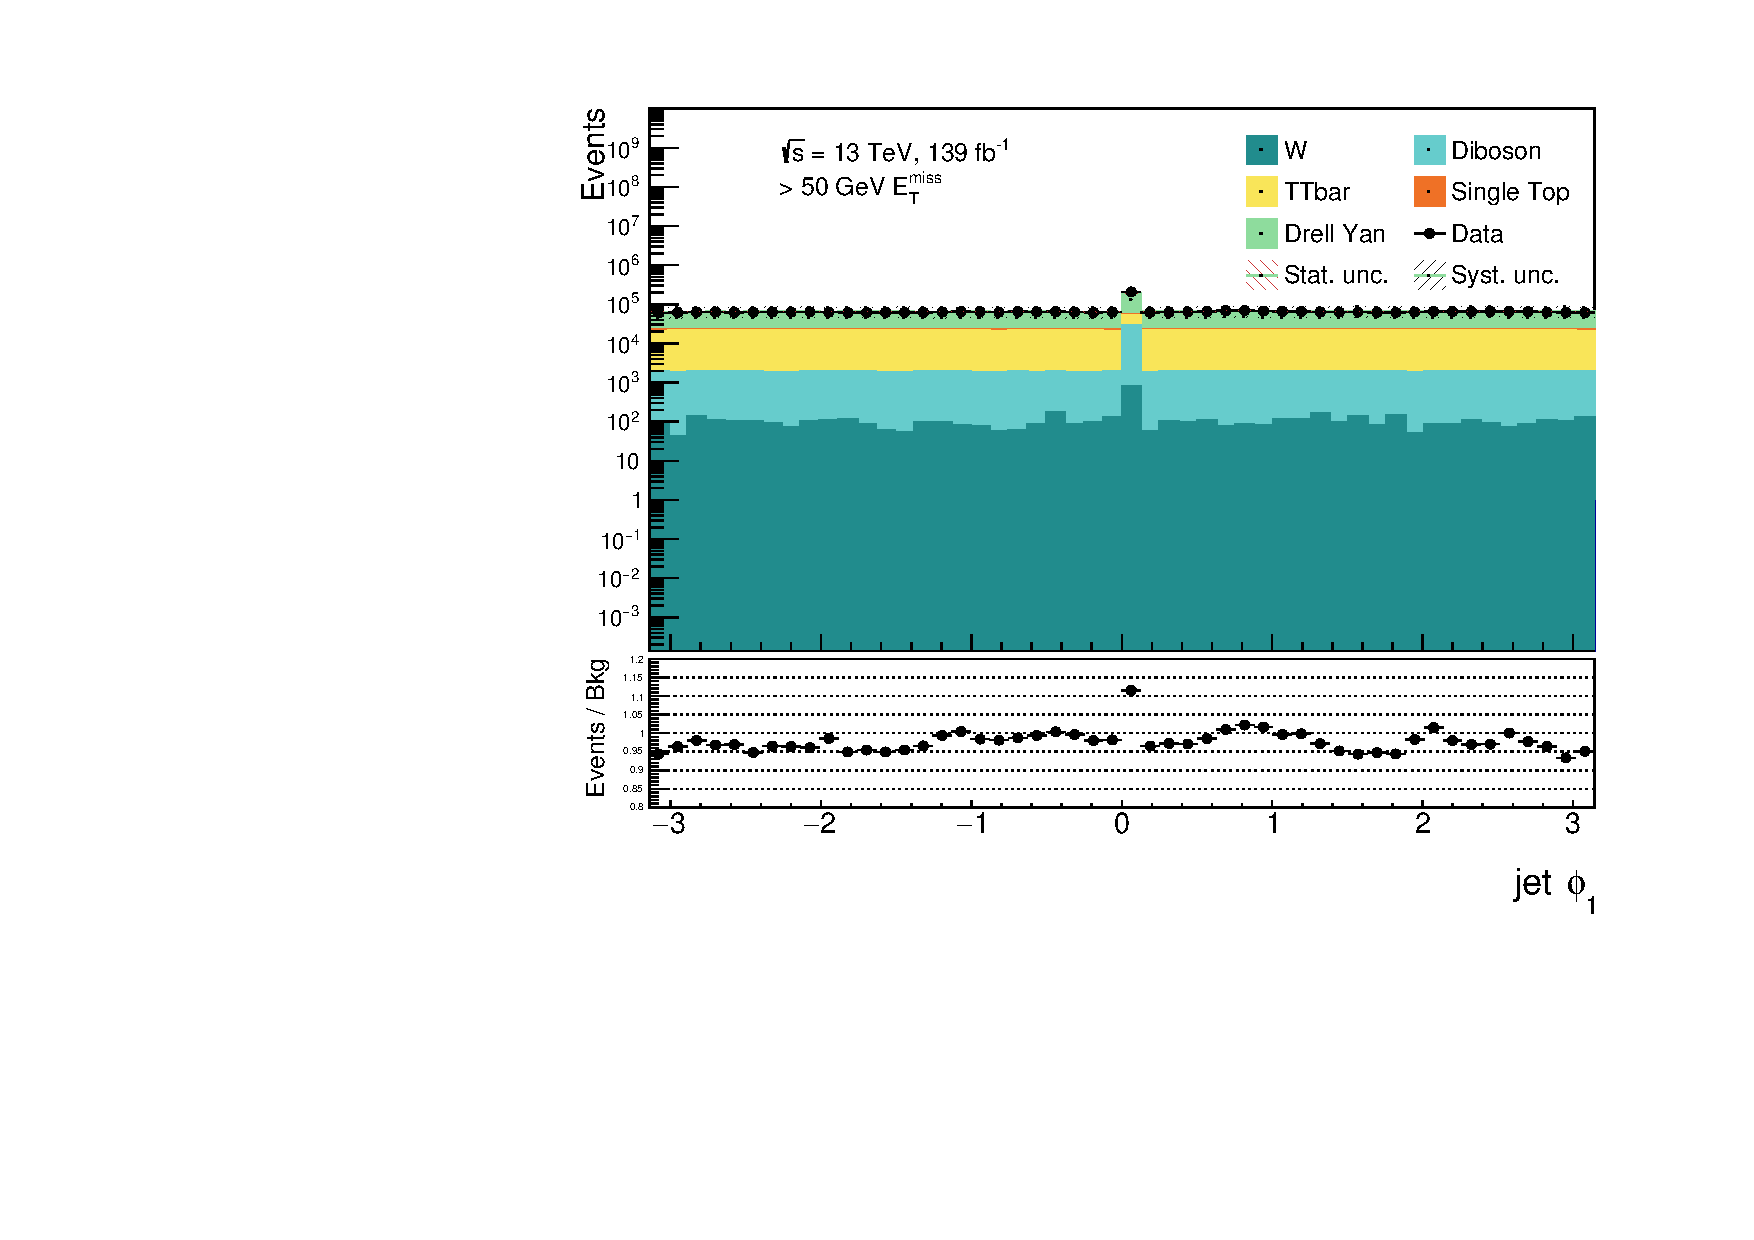
\includegraphics[width=\textwidth]{phi1_jet.pdf}
    \end{subfigure}
    \hfill
    \begin{subfigure}[b]{0.49\textwidth}
        \centering
        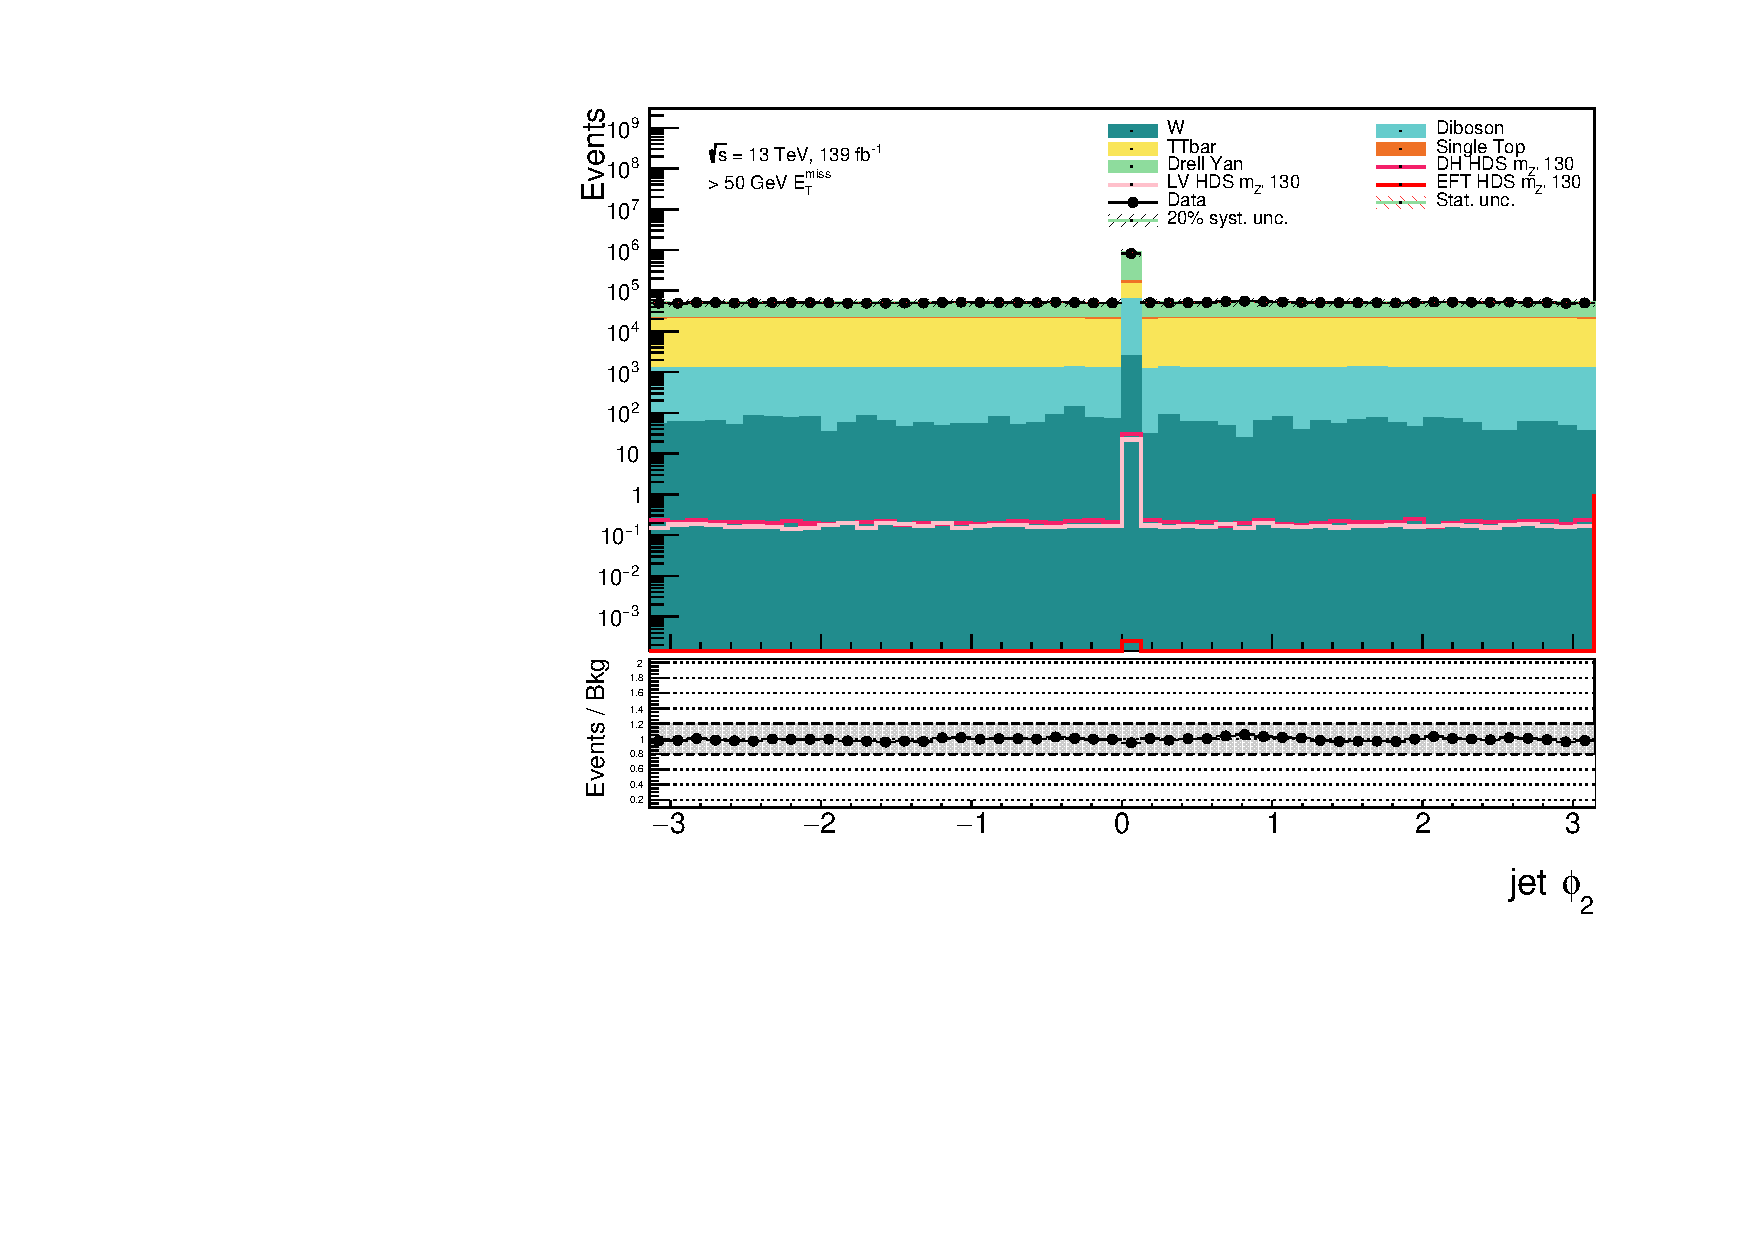
\includegraphics[width=\textwidth]{phi2_jet.pdf}
    \end{subfigure}
    \begin{subfigure}[b]{0.49\textwidth}
        \centering
        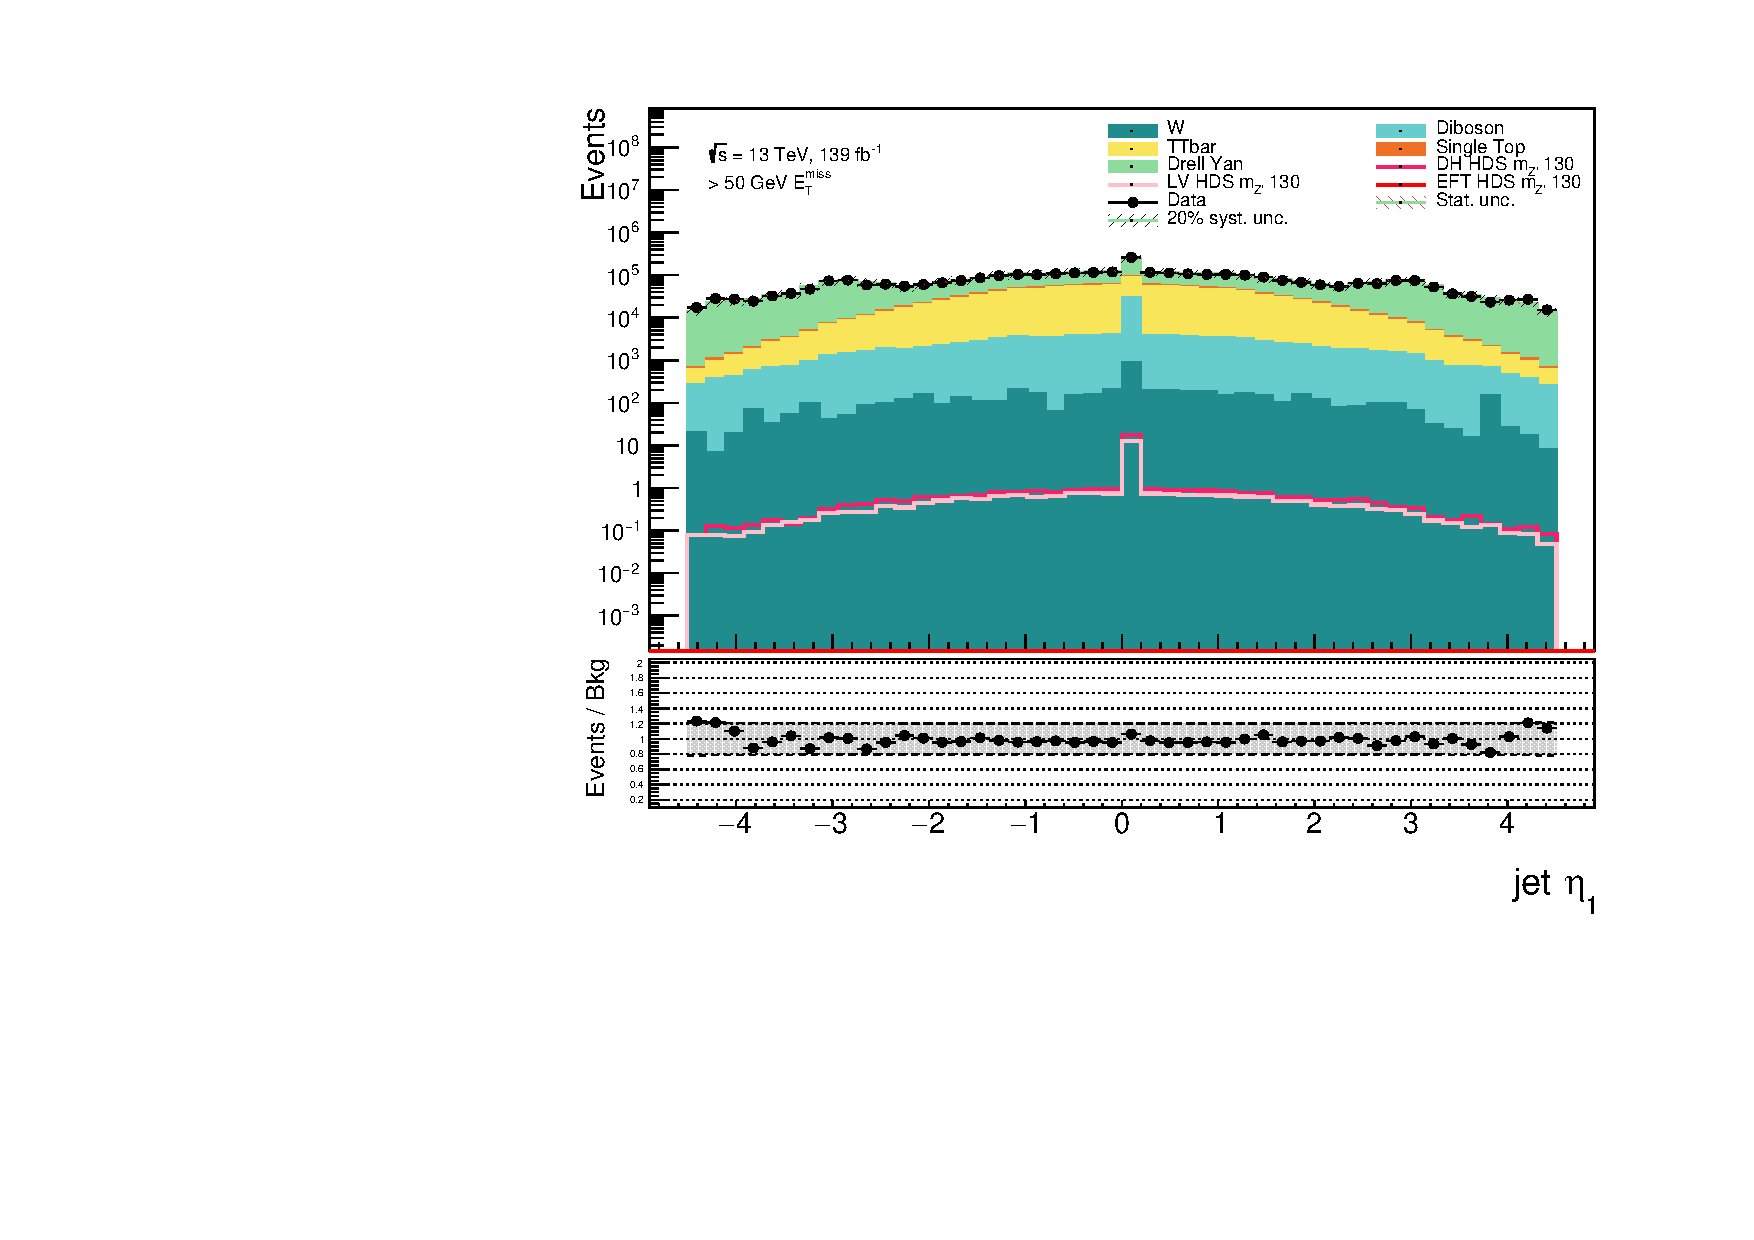
\includegraphics[width=\textwidth]{eta1_jet.pdf}
    \end{subfigure}
    \hfill
    \begin{subfigure}[b]{0.49\textwidth}
        \centering
        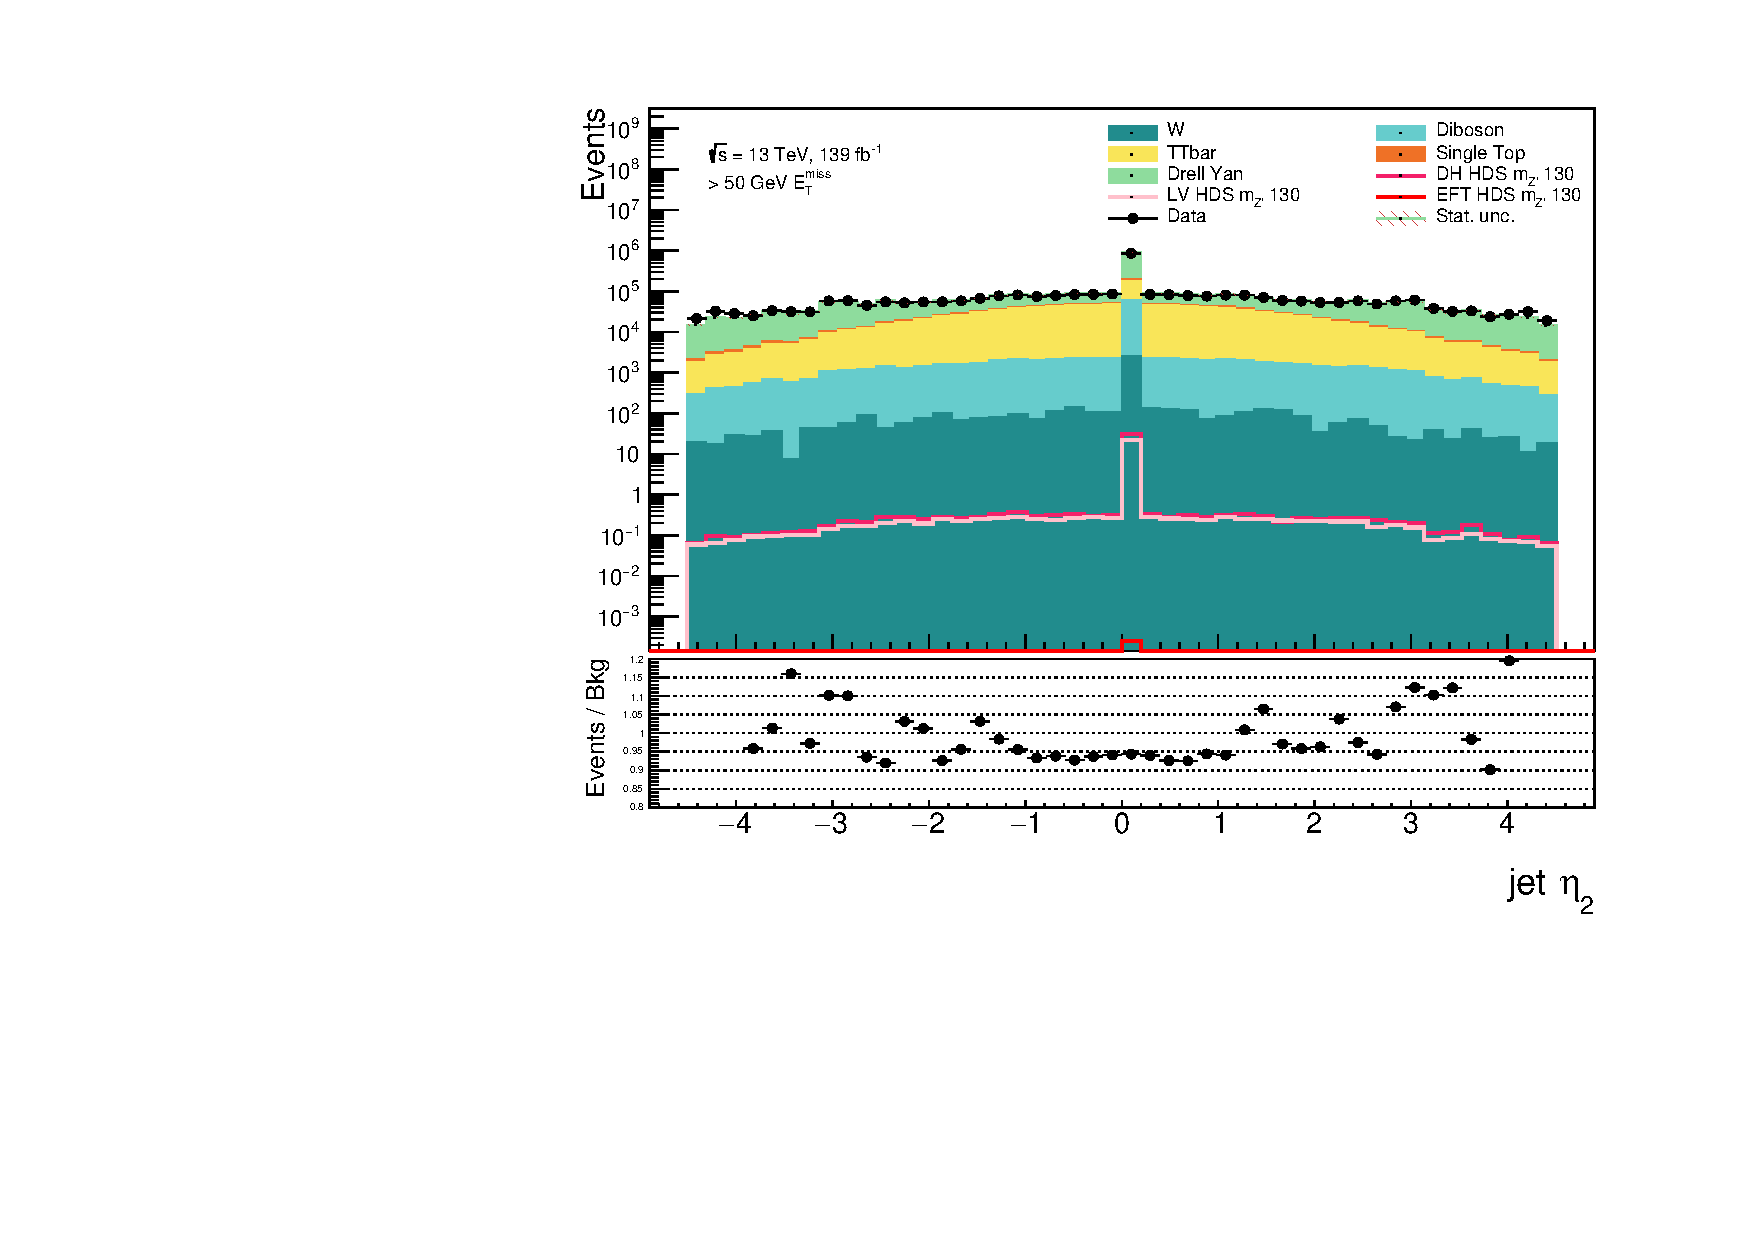
\includegraphics[width=\textwidth]{eta2_jet.pdf}
    \end{subfigure}
    \caption{Leading jets $p_T, \phi$ and $\eta$ distribution in the control region.}
\end{figure}
\begin{figure}[!ht]
    \centering
    \begin{subfigure}[b]{0.49\textwidth}
        \centering
        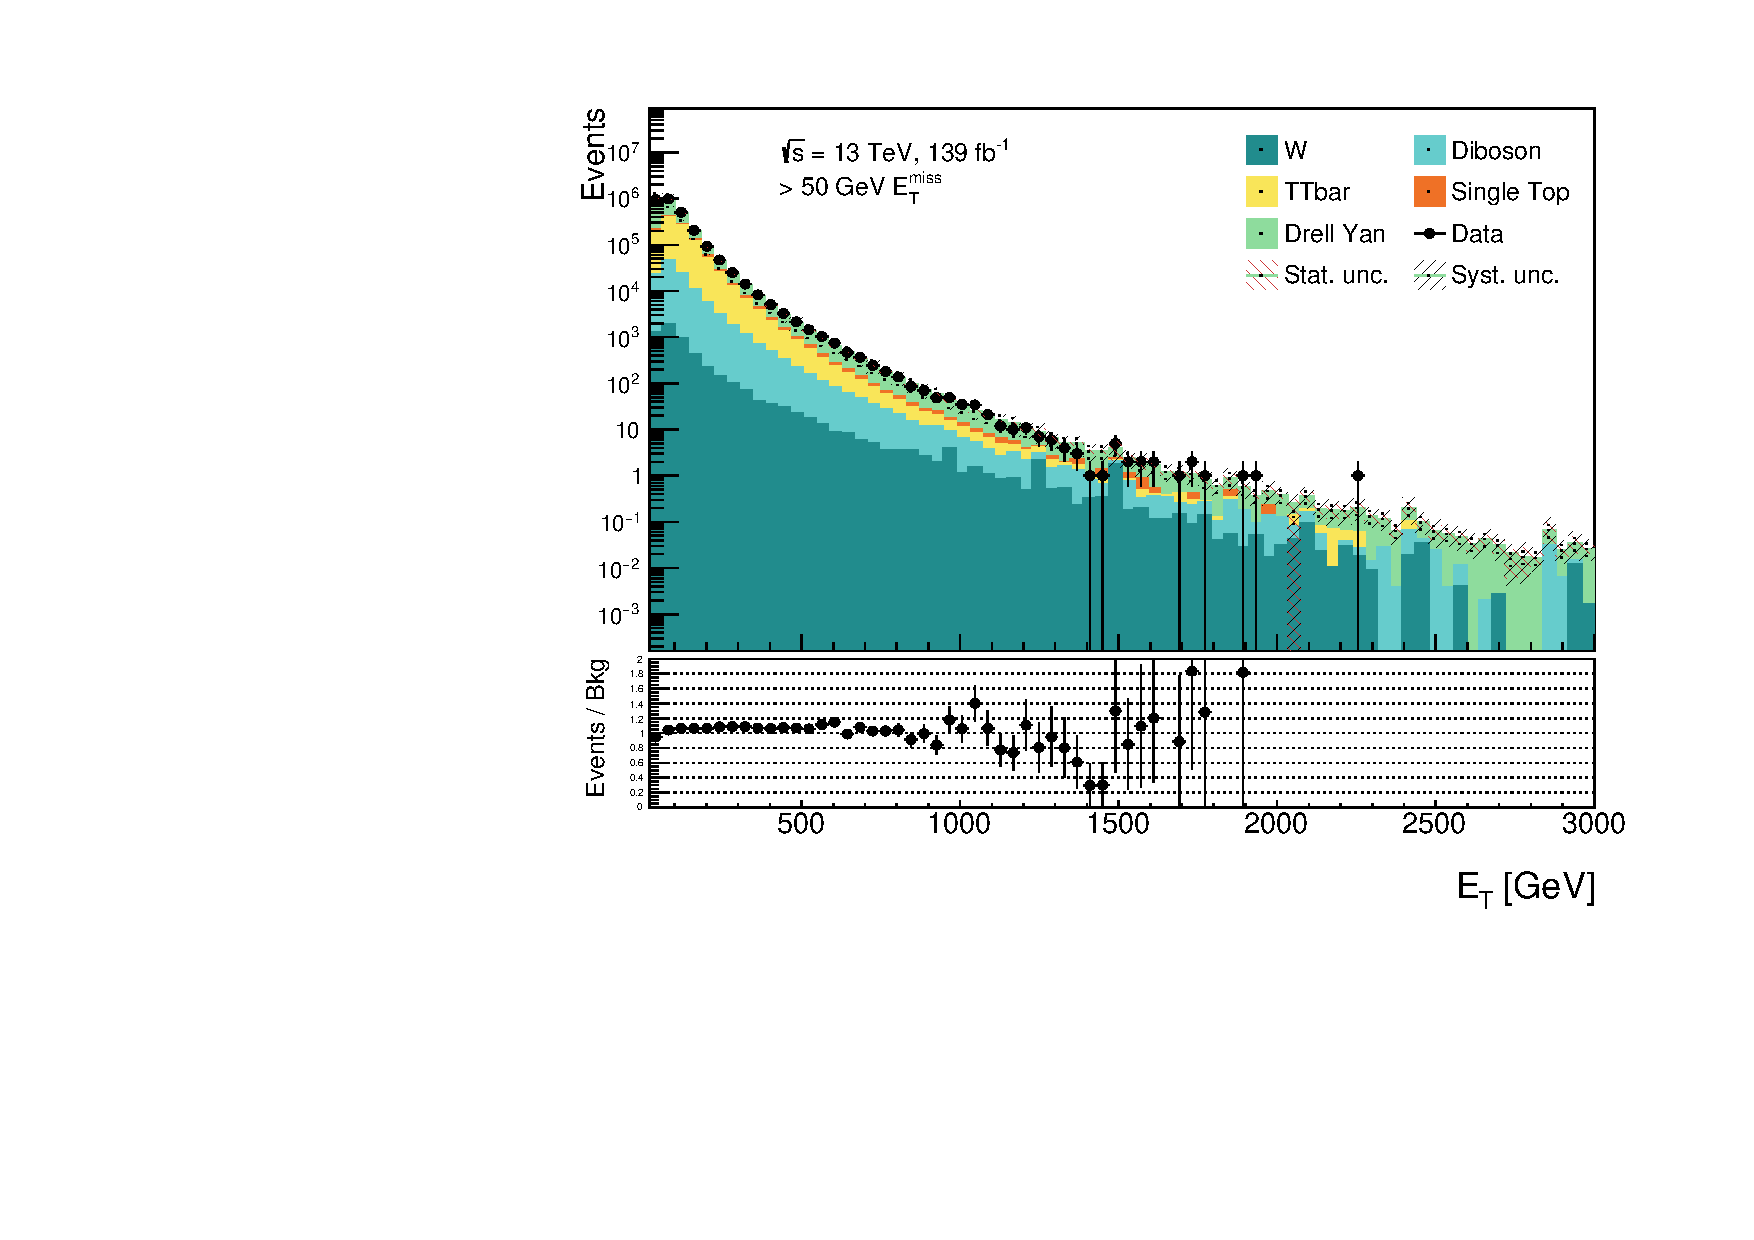
\includegraphics[width=\textwidth]{et.pdf}
    \end{subfigure}
    \hfill
    \begin{subfigure}[b]{0.49\textwidth}
        \centering
        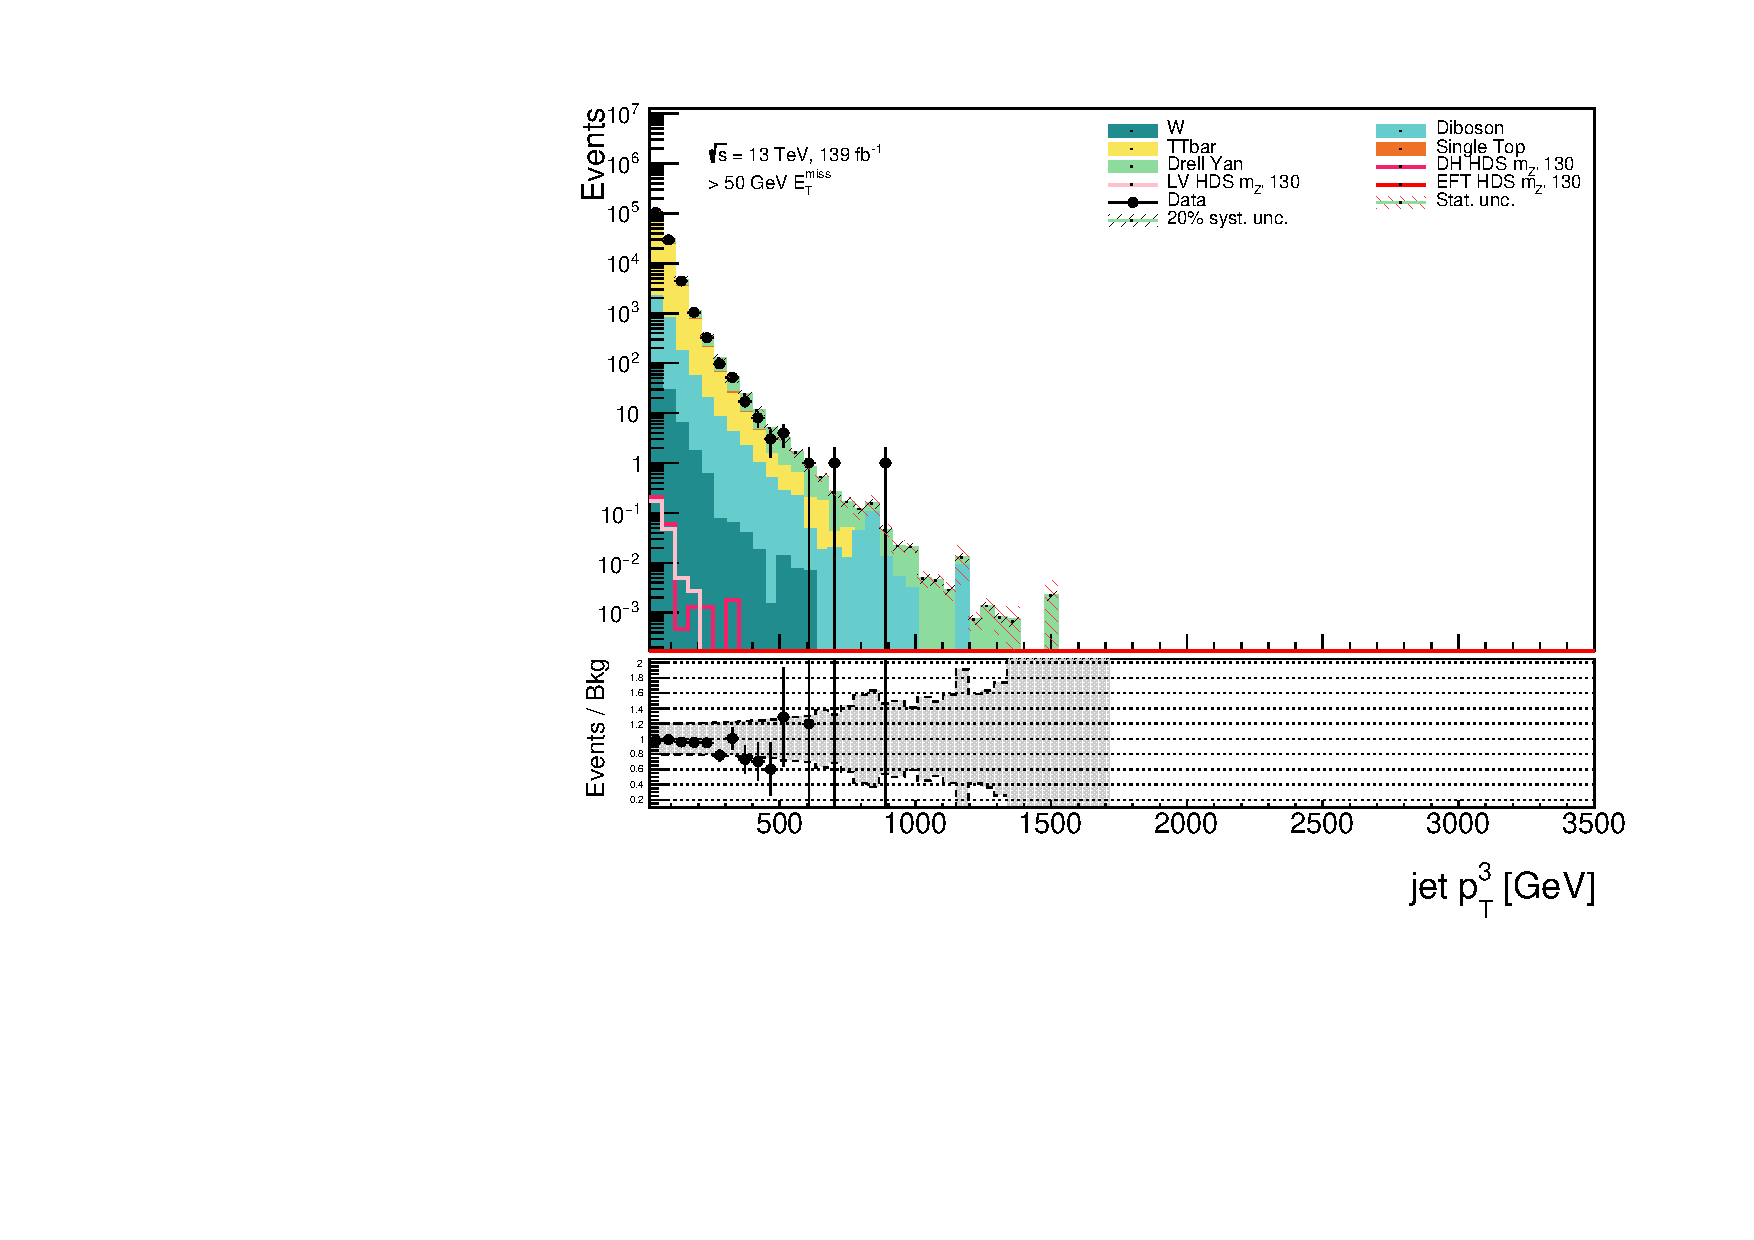
\includegraphics[width=\textwidth]{pt3_jet.pdf}
    \end{subfigure}
    \begin{subfigure}[b]{0.49\textwidth}
        \centering
        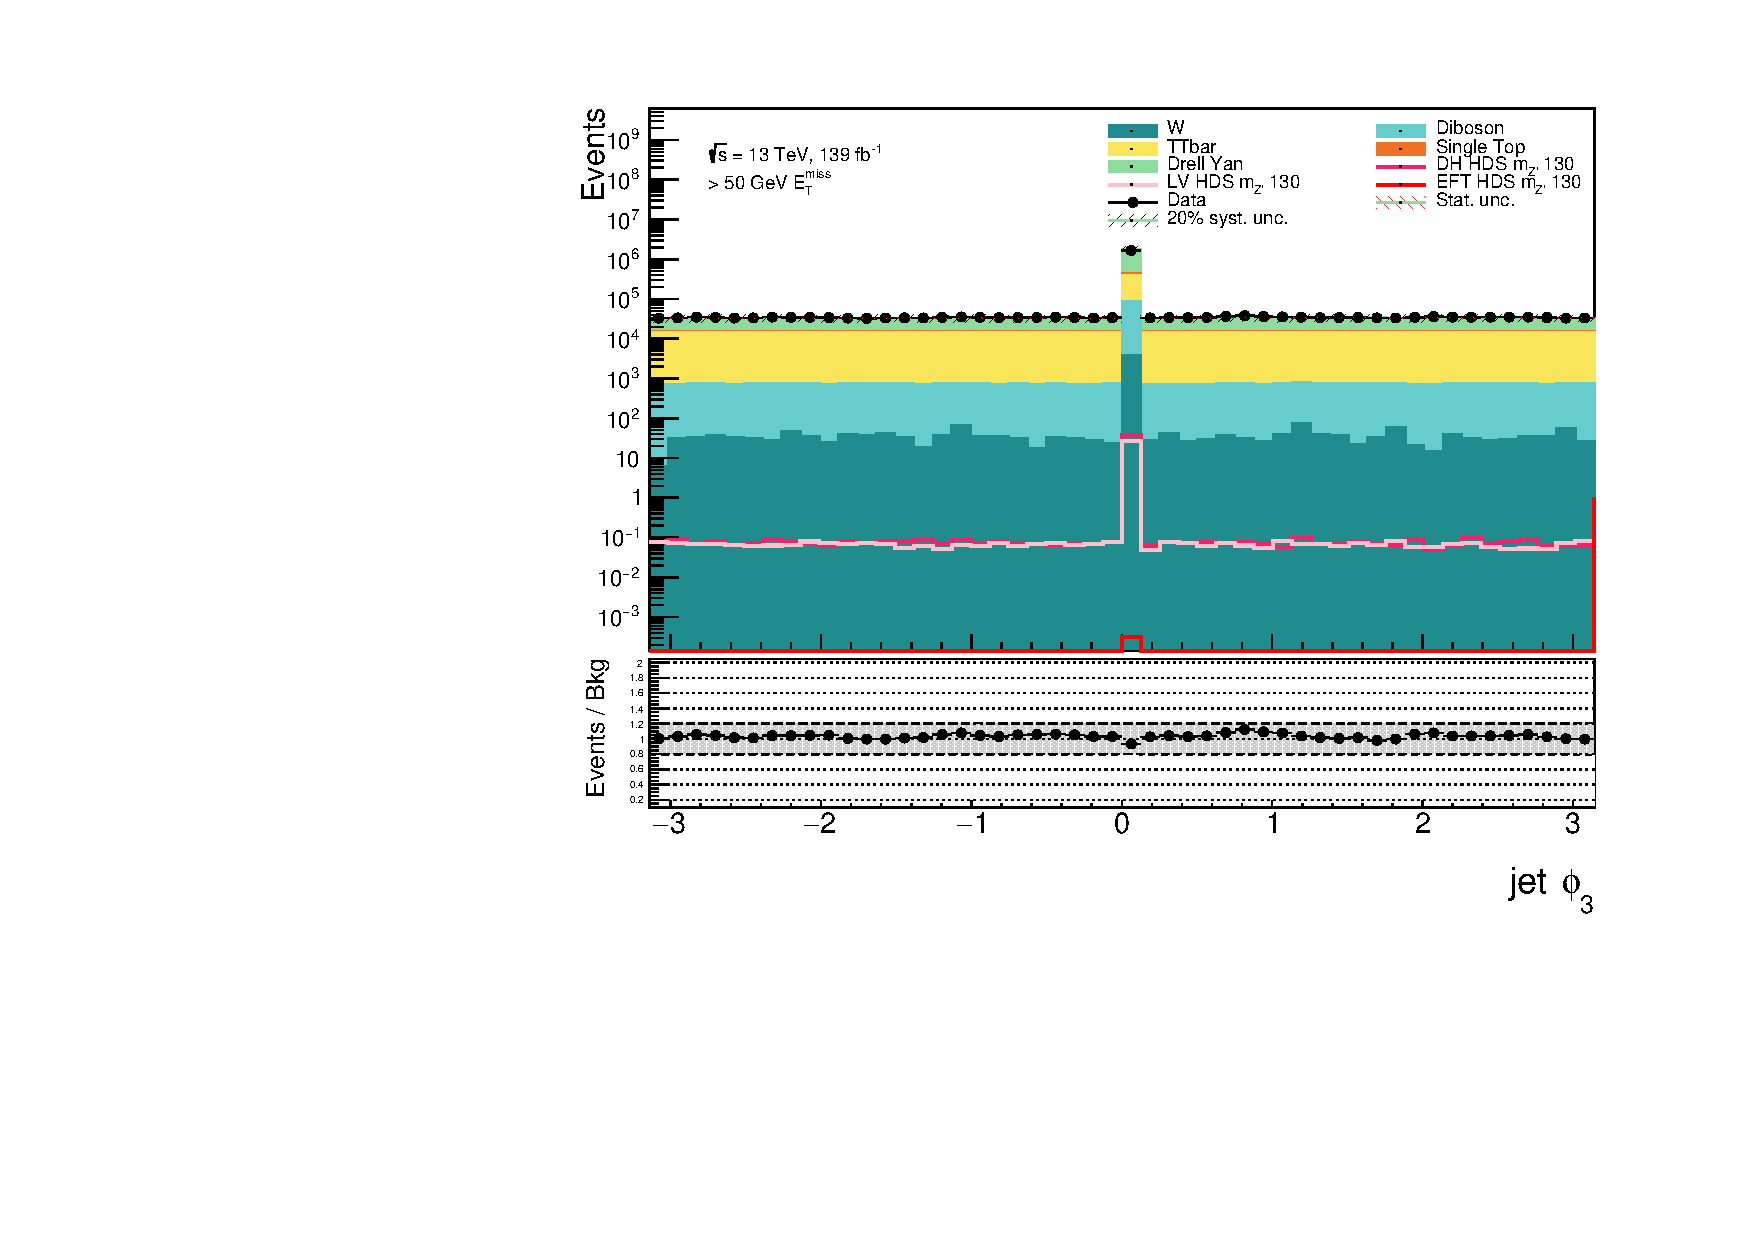
\includegraphics[width=\textwidth]{phi3_jet.pdf}
    \end{subfigure}
    \begin{subfigure}[b]{0.49\textwidth}
        \centering
        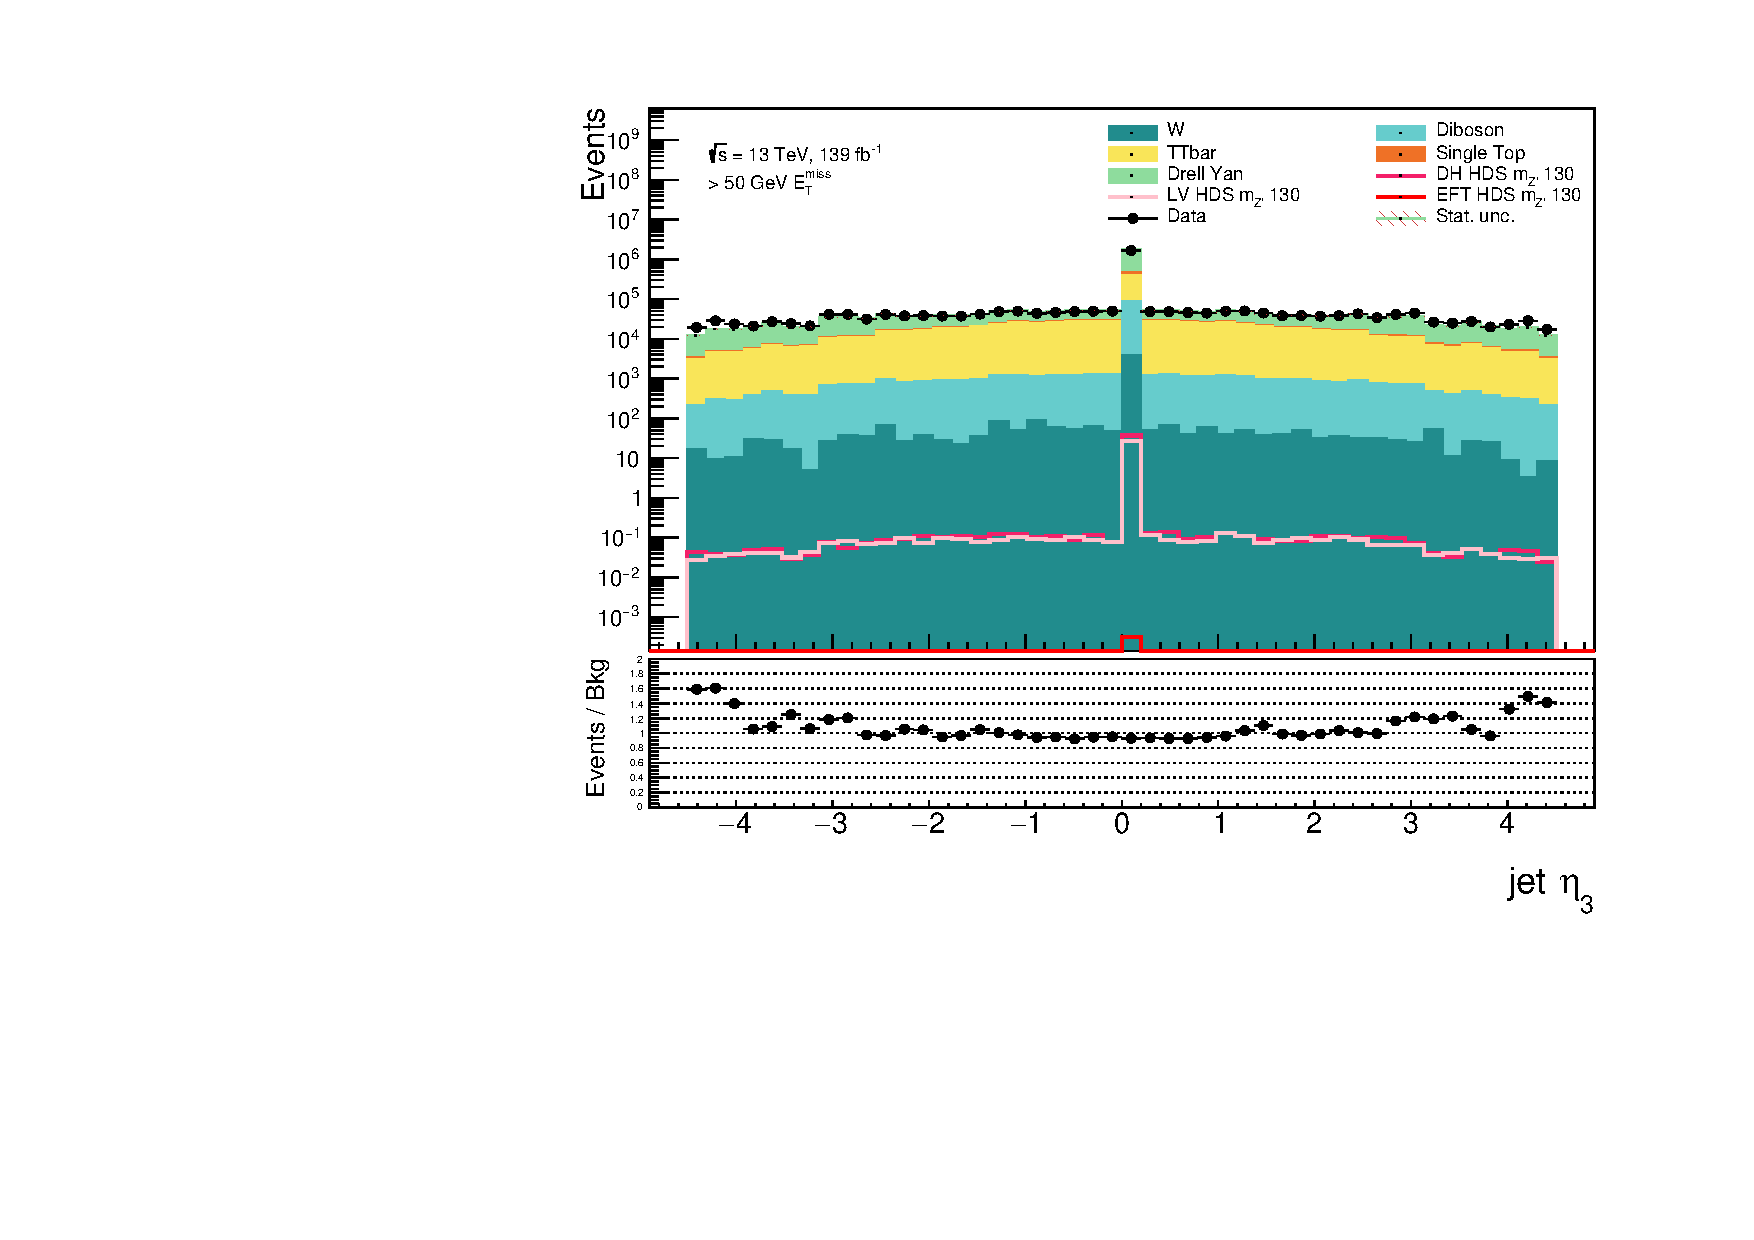
\includegraphics[width=\textwidth]{eta3_jet.pdf}
    \end{subfigure}
    \begin{subfigure}[b]{0.49\textwidth}
        \centering
        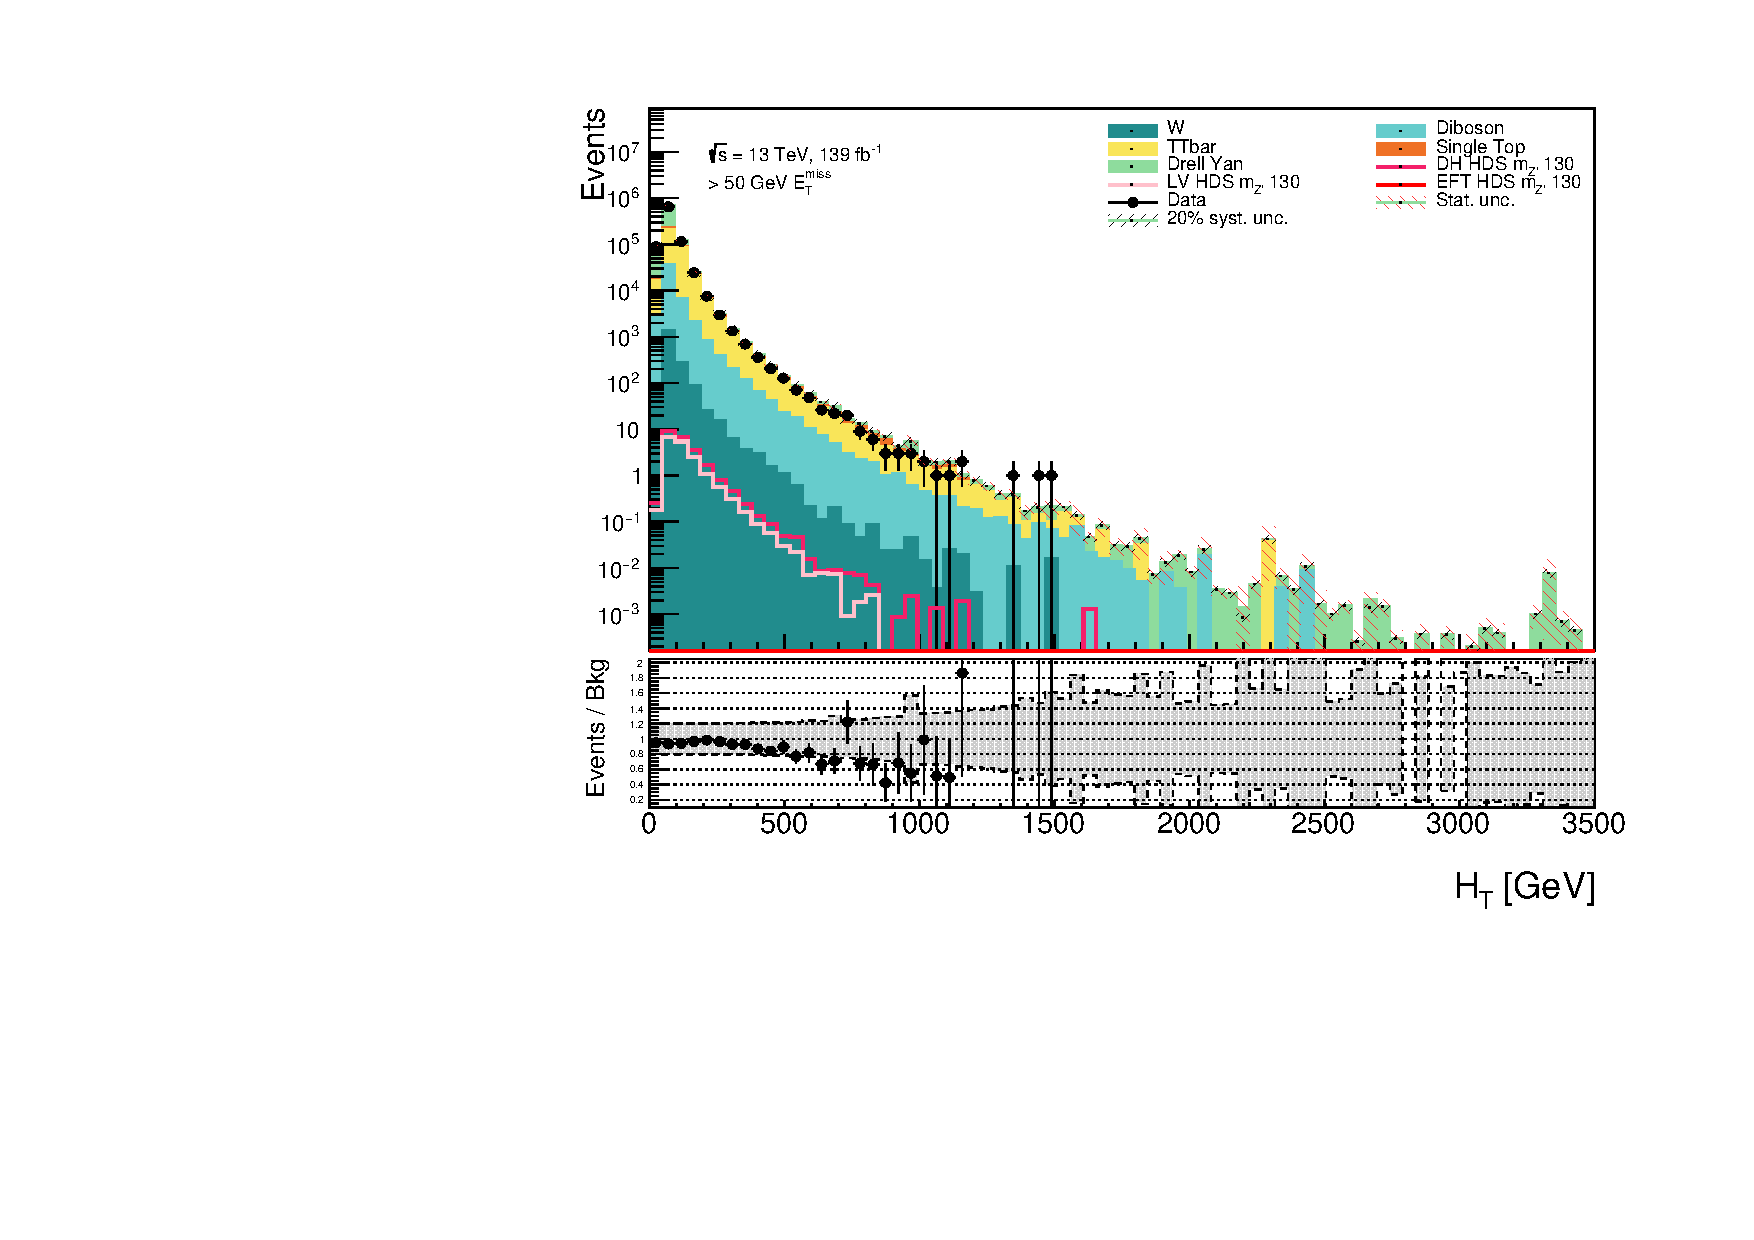
\includegraphics[width=\textwidth]{ht.pdf}
    \end{subfigure}
    \begin{subfigure}[b]{0.49\textwidth}
        \centering
        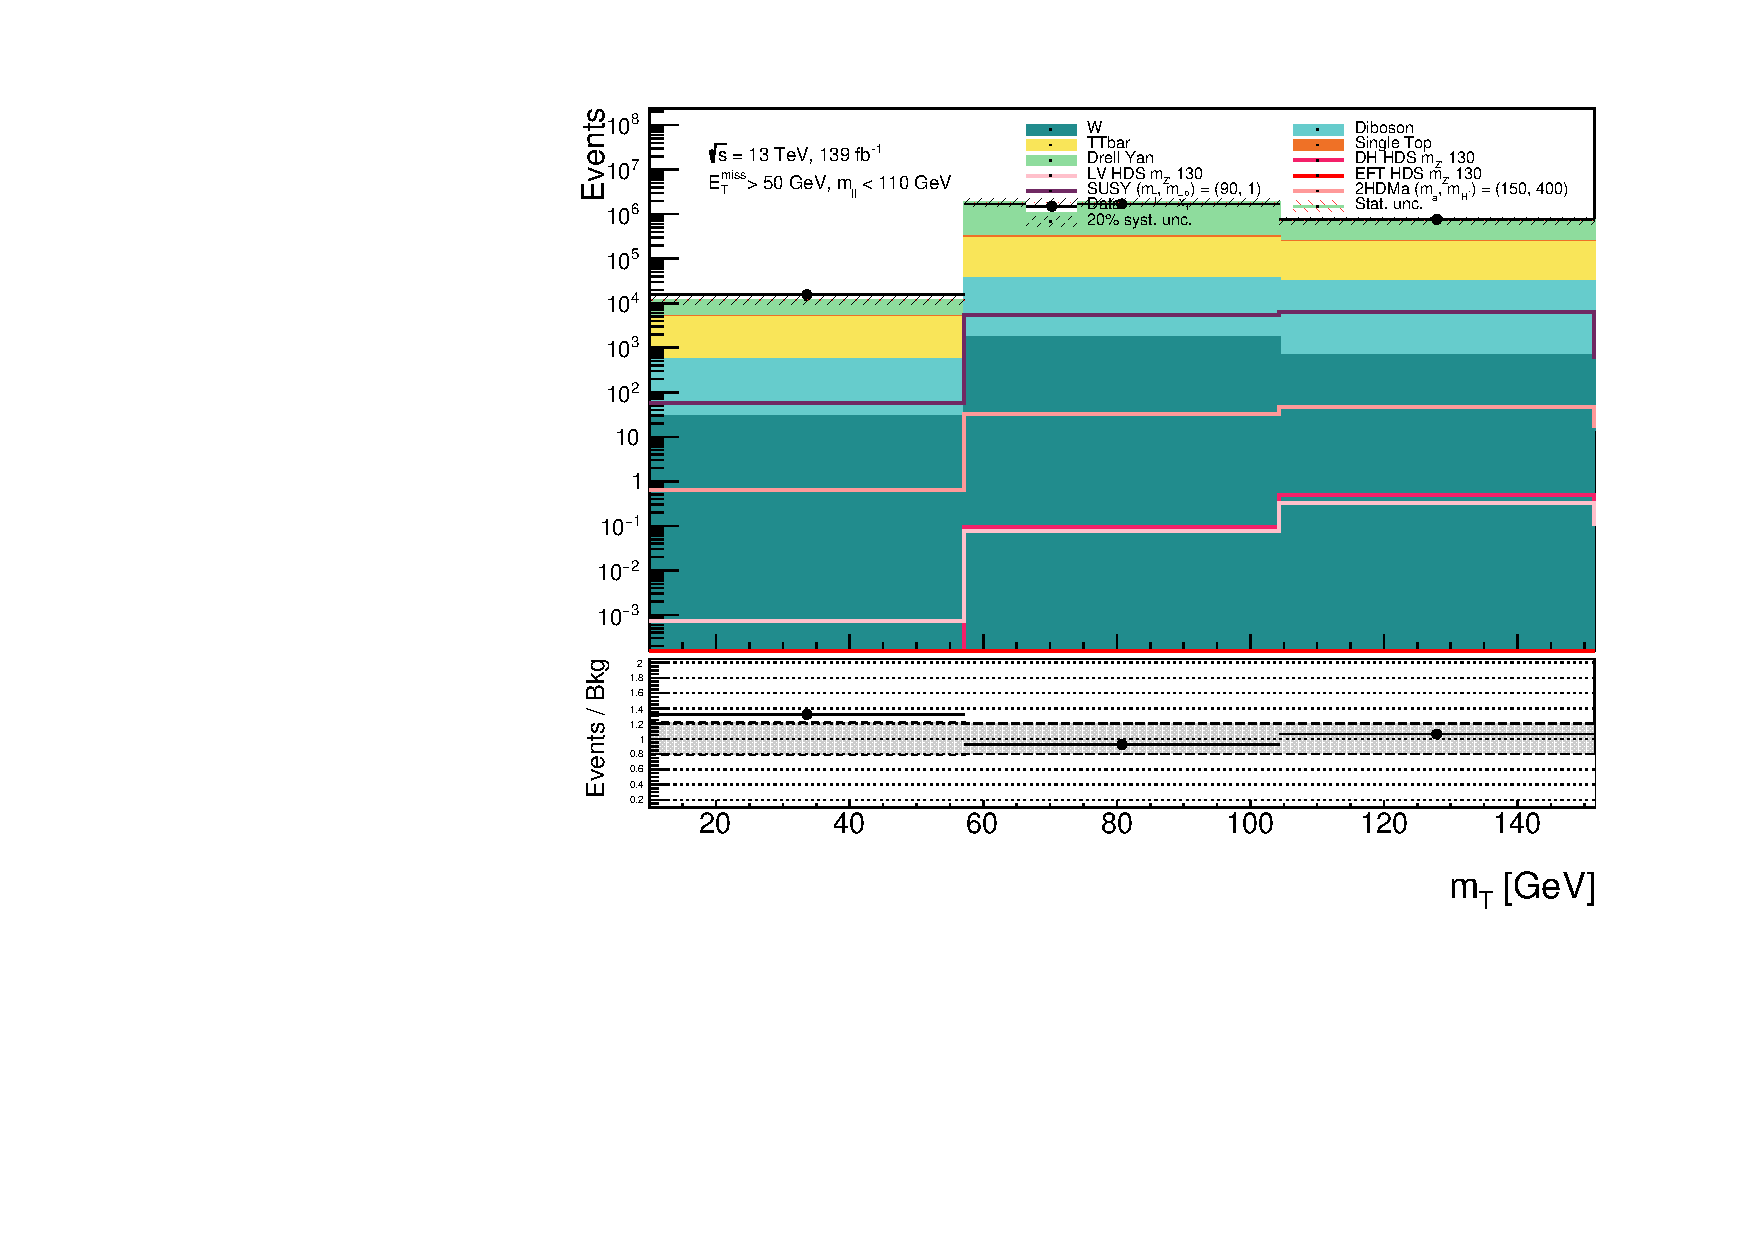
\includegraphics[width=\textwidth]{mt.pdf}
    \end{subfigure}
    \caption{$p_T, \phi$ and $\eta$ of third leading jet and the dilepton pairs $E_T$, $H_T$ and $m_T$ distribution in the control region.}
\end{figure}
\begin{figure}[!ht]
    \centering
    \begin{subfigure}[b]{0.49\textwidth}
        \centering
        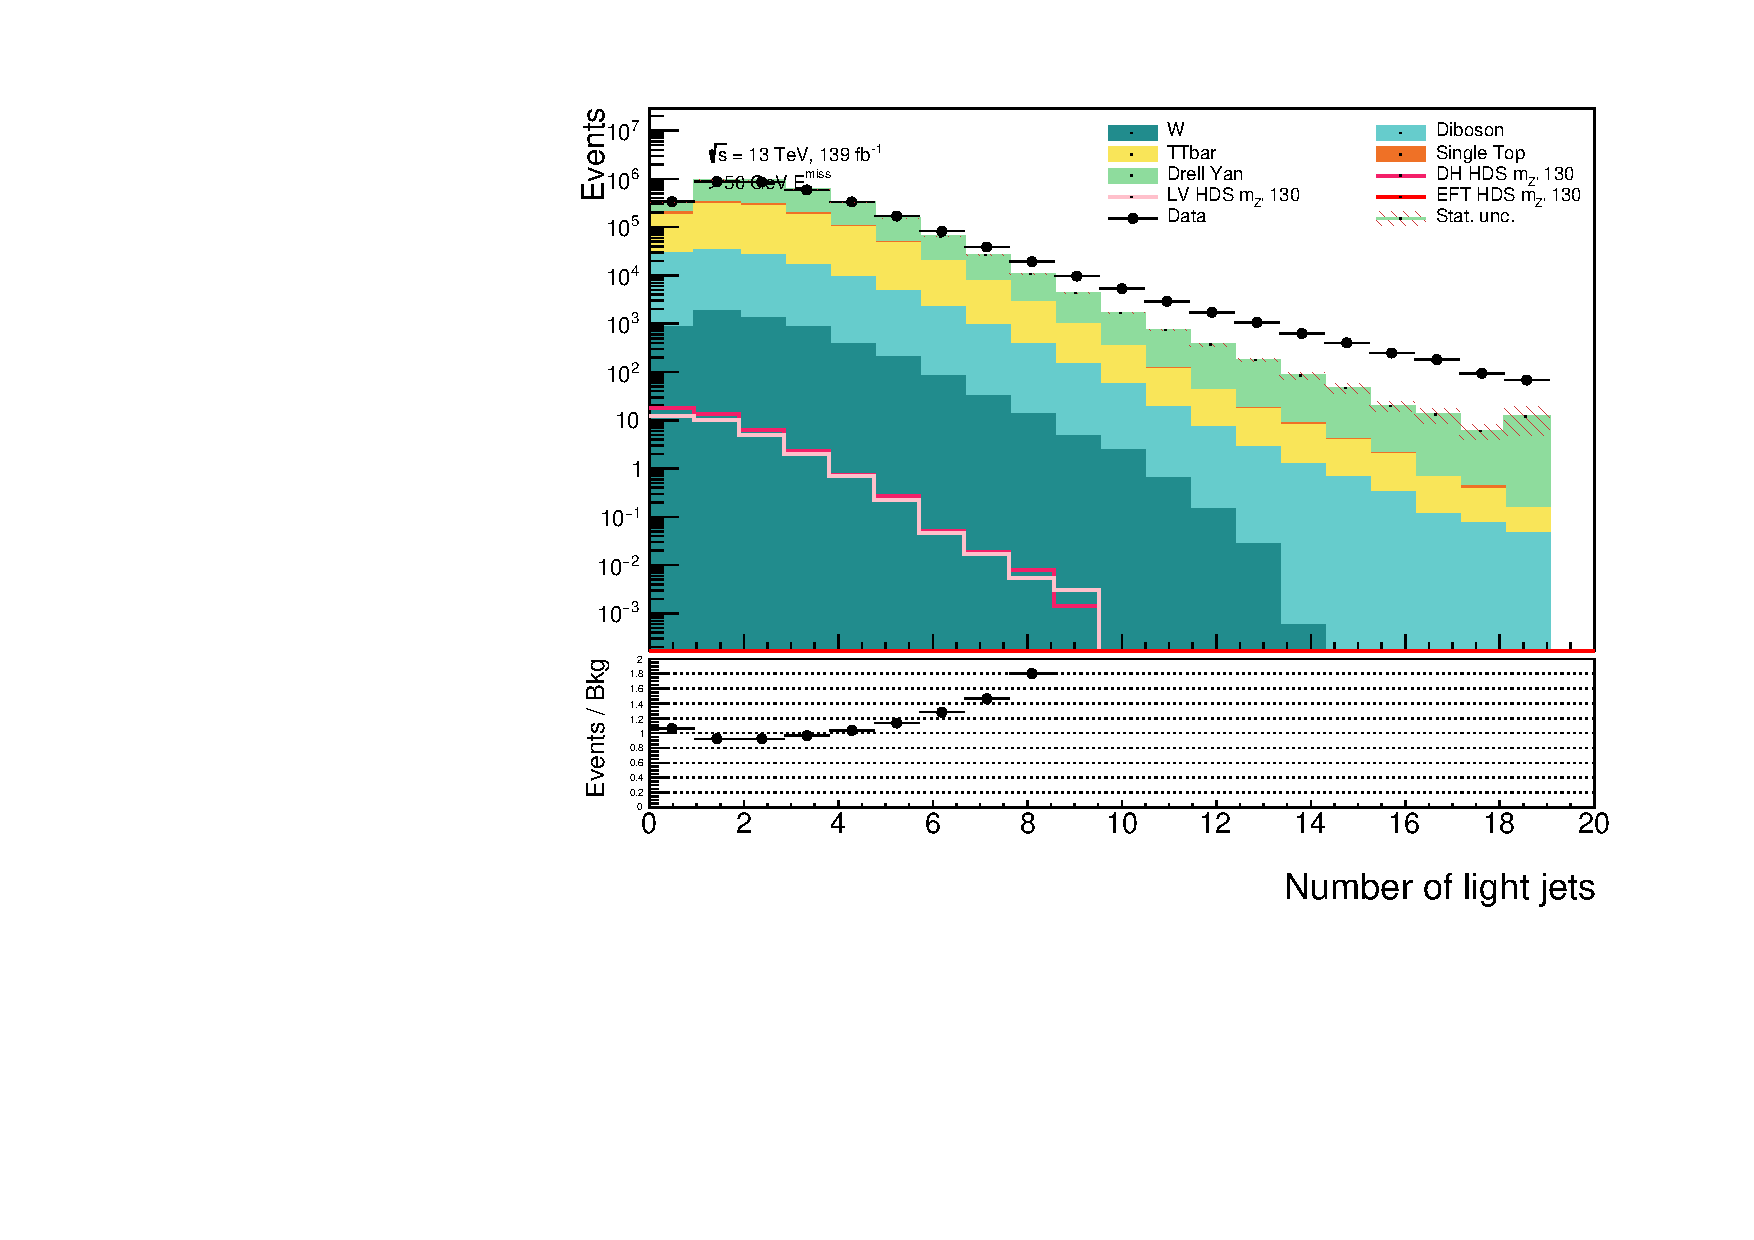
\includegraphics[width=\textwidth]{nLJet.pdf}
    \end{subfigure}
    \hfill
    \begin{subfigure}[b]{0.49\textwidth}
        \centering
        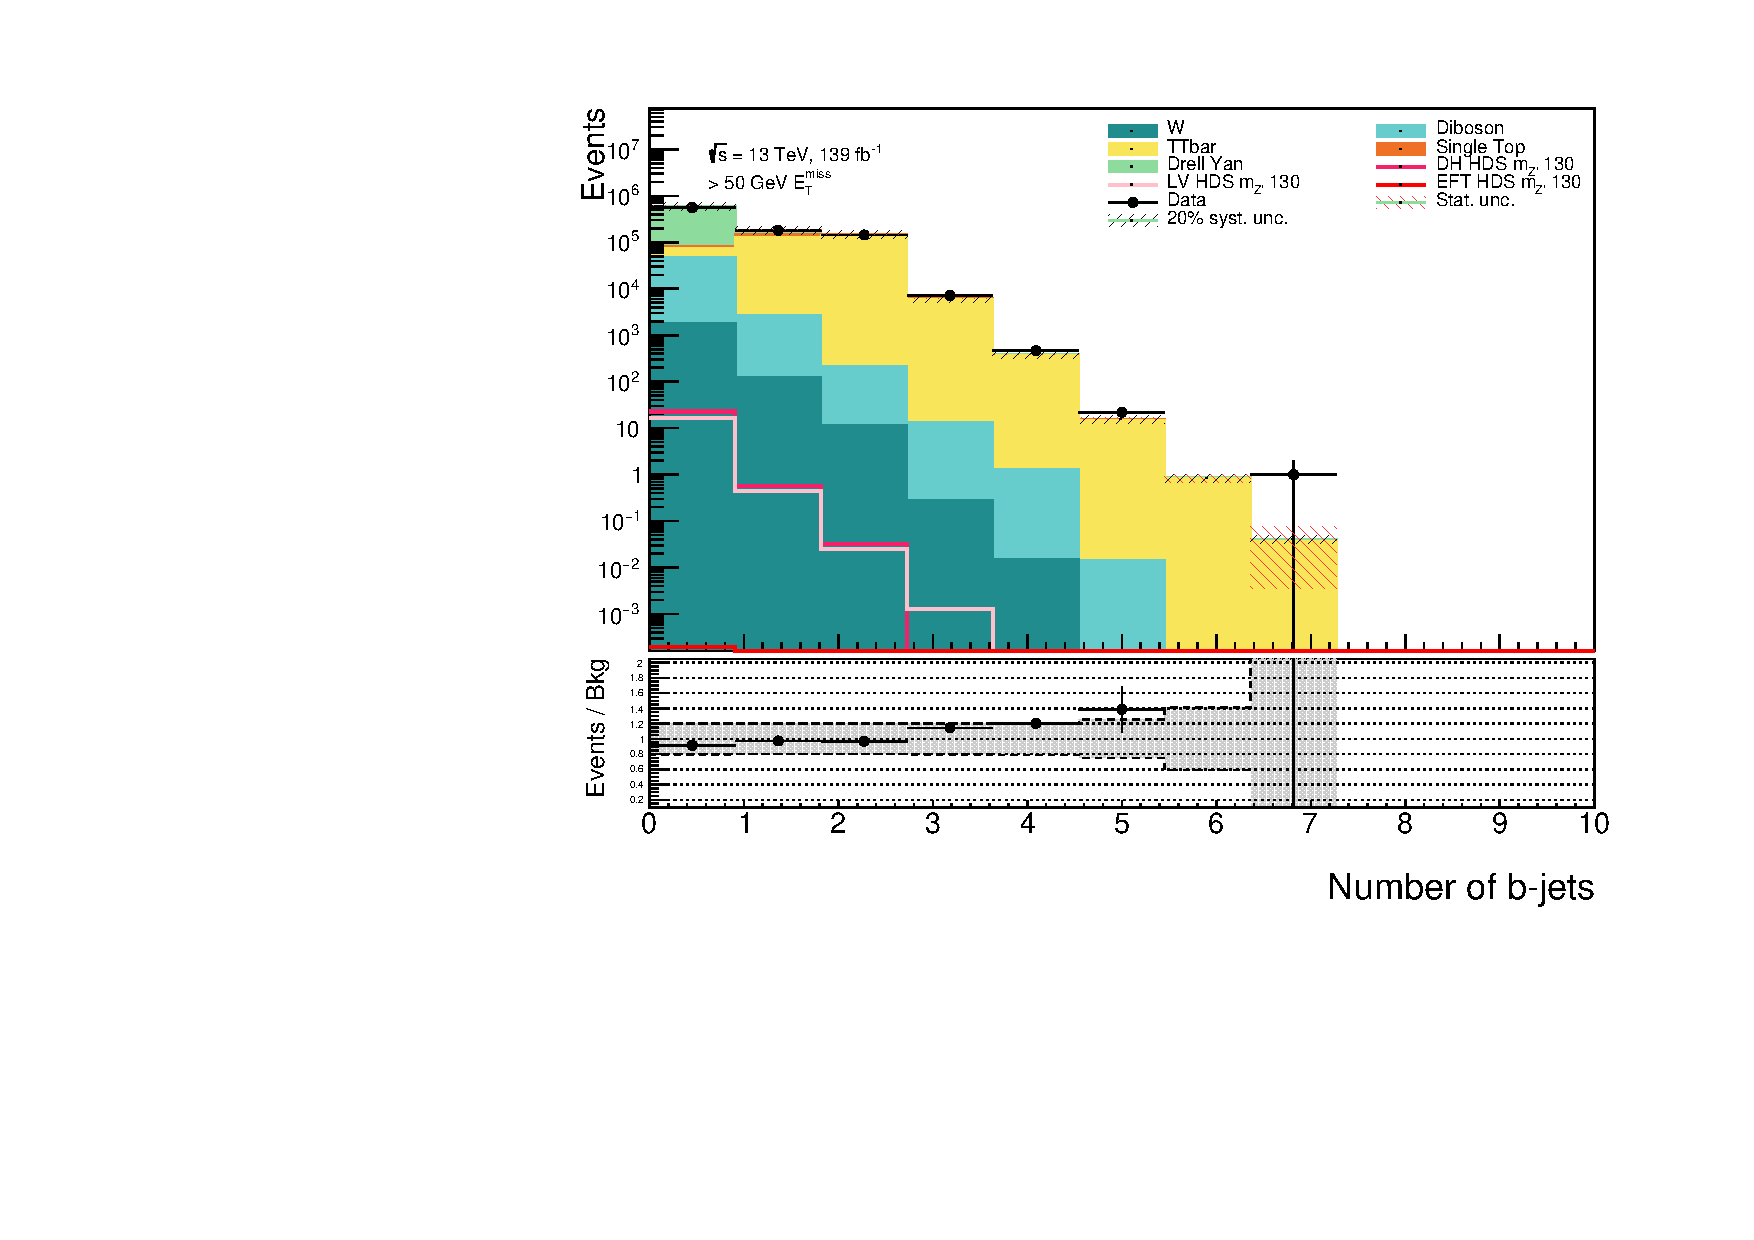
\includegraphics[width=\textwidth]{nBJet.pdf}
    \end{subfigure}
    \hfill
    \begin{subfigure}[b]{0.49\textwidth}
        \centering
        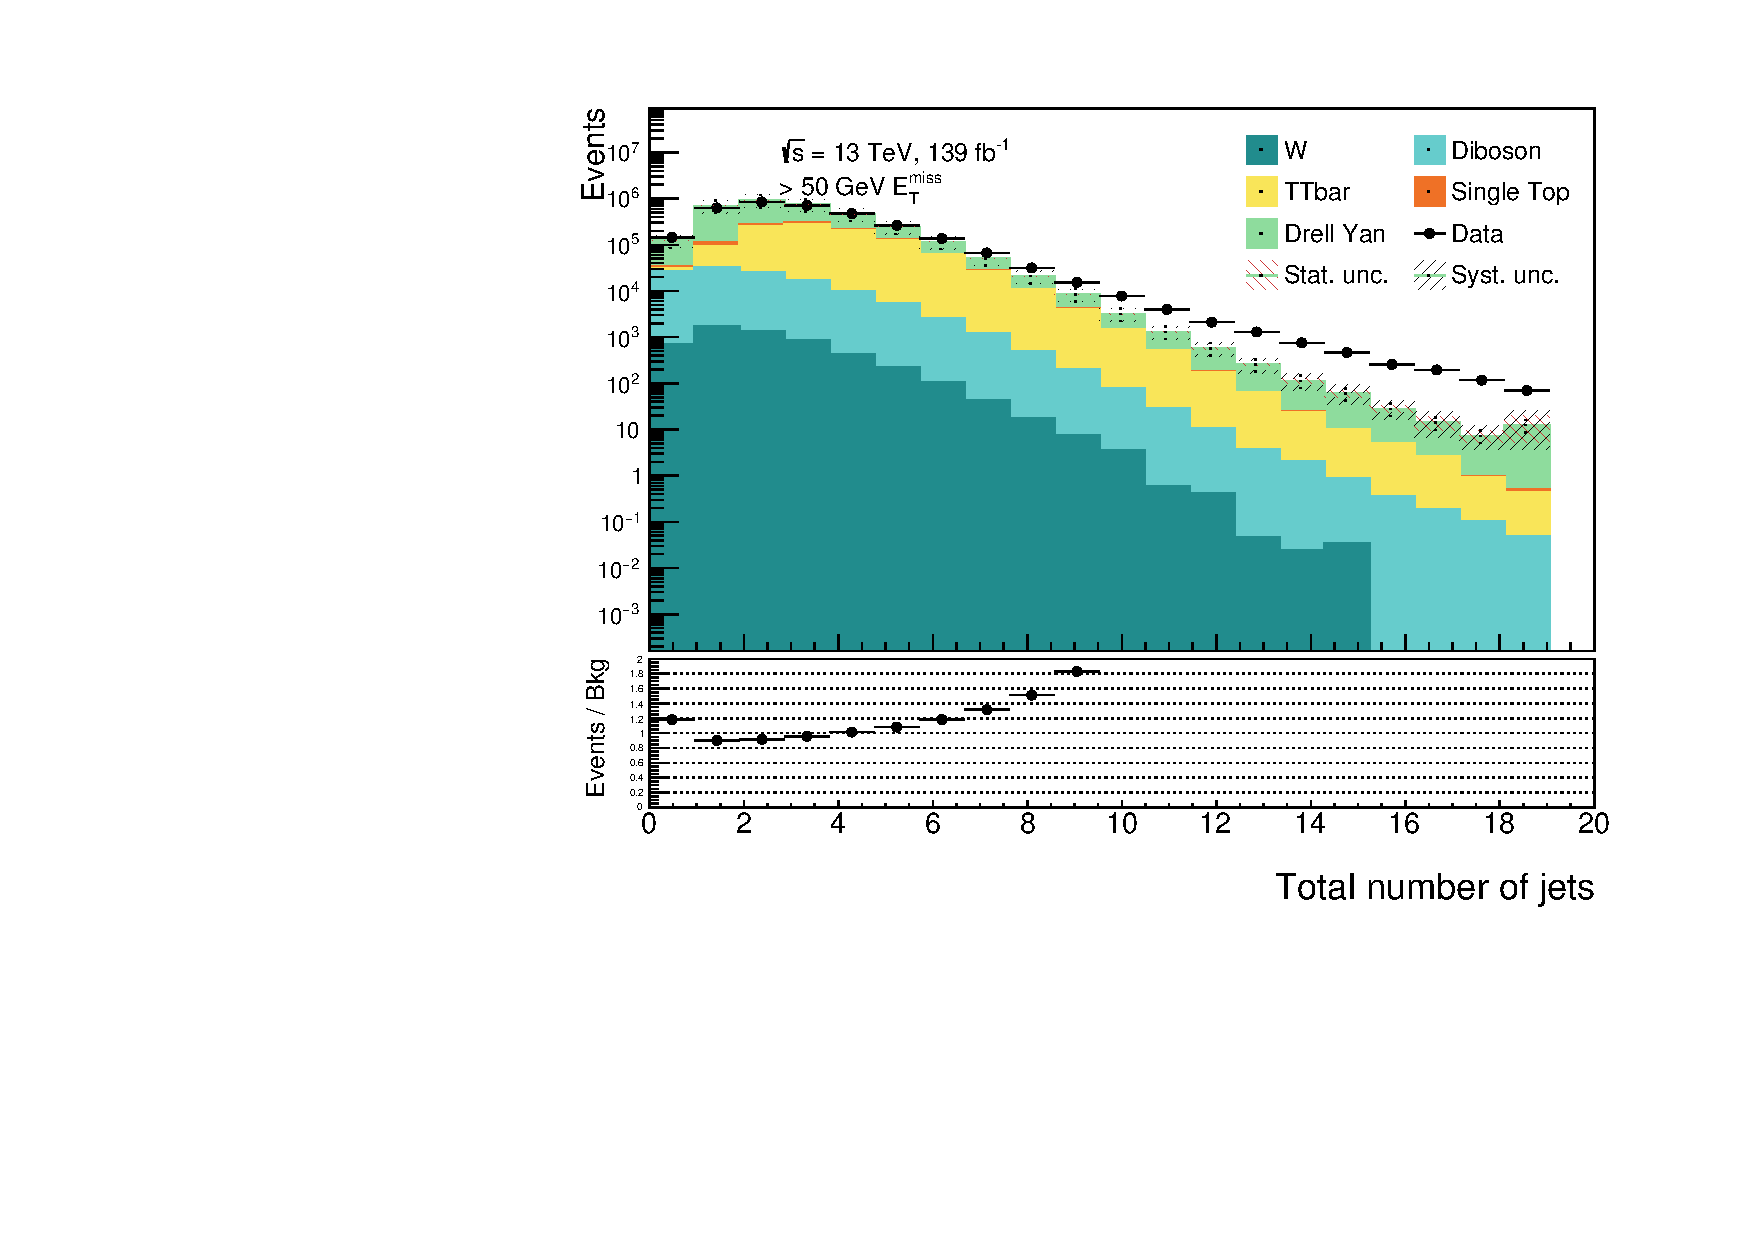
\includegraphics[width=\textwidth]{nTJet.pdf}
    \end{subfigure}
    \hfill
    \begin{subfigure}[b]{0.49\textwidth}
        \centering
        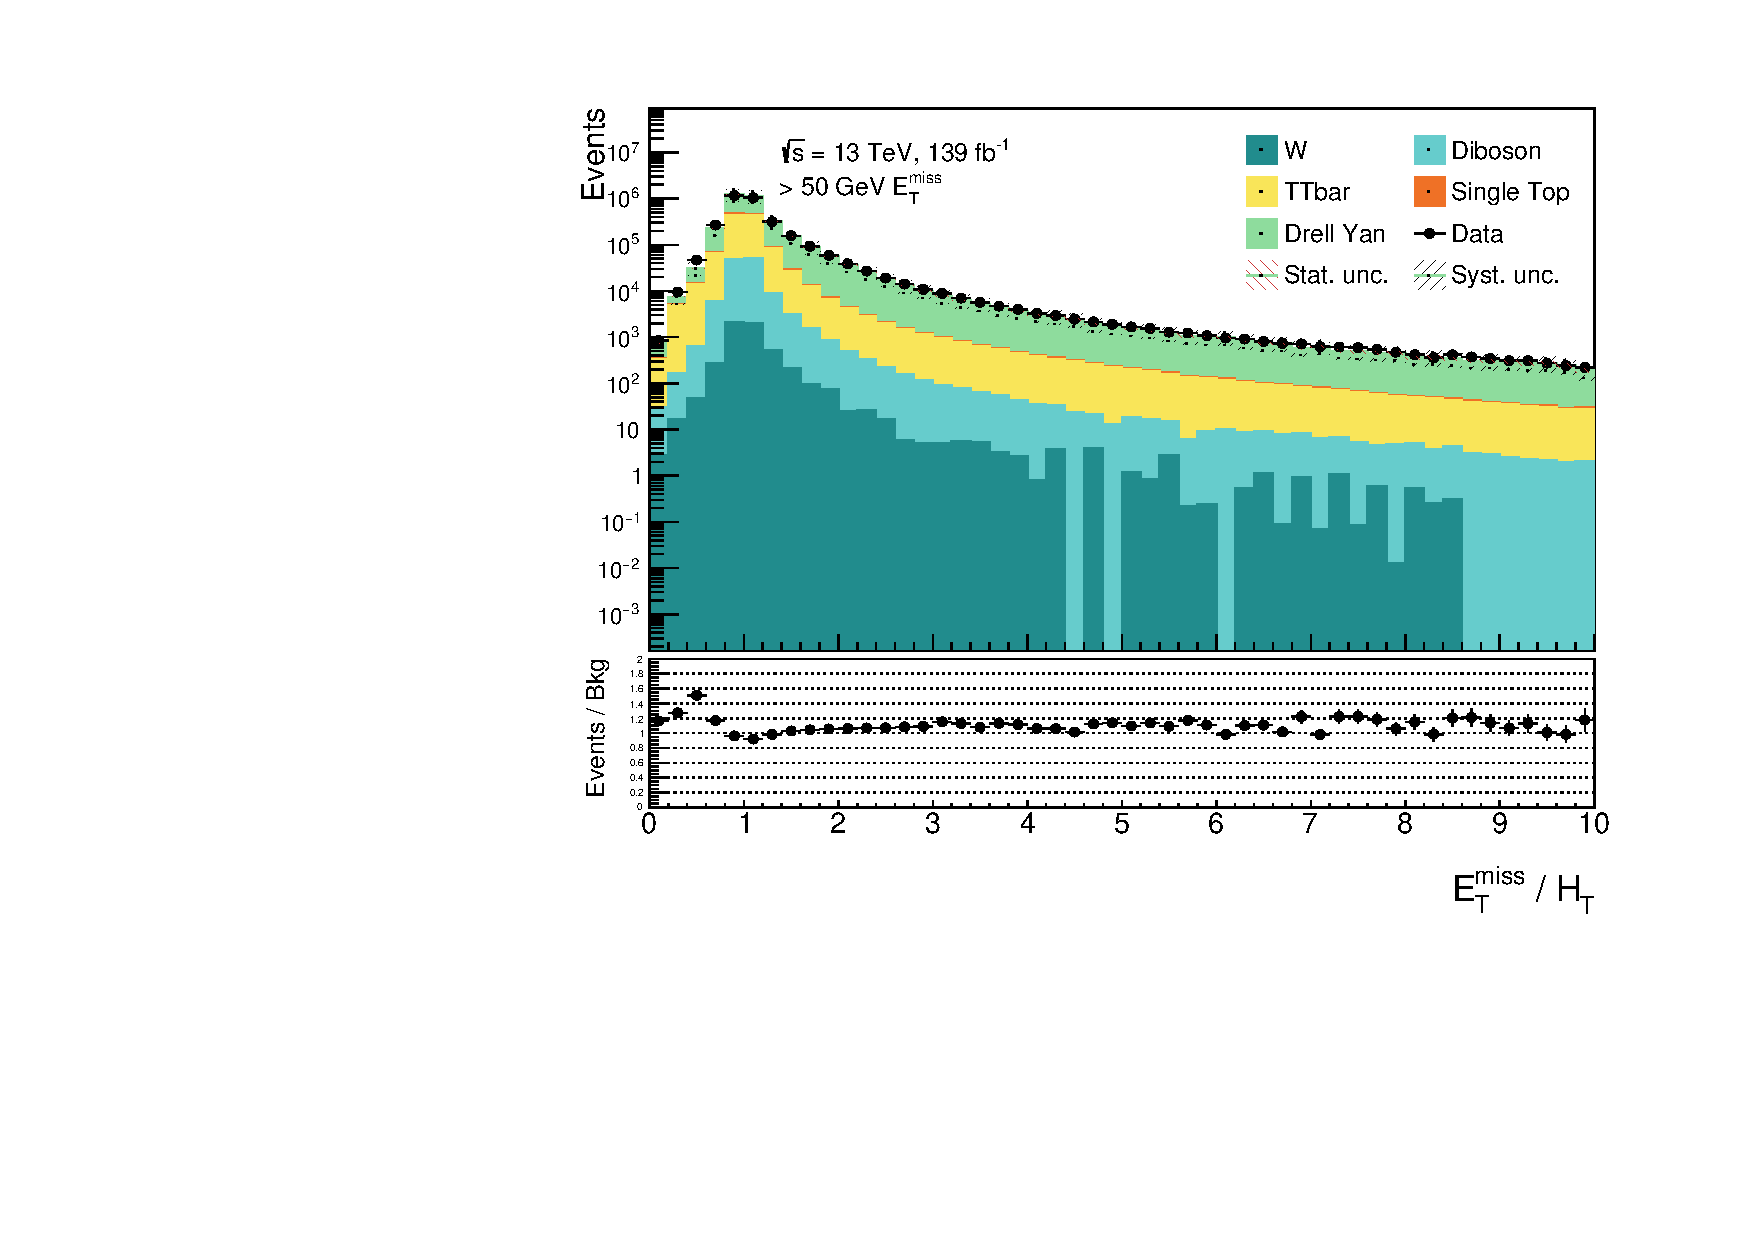
\includegraphics[width=\textwidth]{rt.pdf}
    \end{subfigure}
    \caption{Number of light, b- and total jets and $E_T^{miss}/H_T$ distribution in the control region.}
\end{figure}

\clearpage


\end{document}